% Paquets généraux
\documentclass[a4paper,12pt,titlepage]{article}
\usepackage[T1]{fontenc}
\usepackage[utf8]{inputenc}
\usepackage[french]{babel}
\usepackage[gen]{eurosym}
%\usepackage[dvips]{graphicx}
\usepackage{fancyhdr}
\usepackage{pdfpages} 
\usepackage{multido}
\usepackage{hyperref}
%\usepackage{textcomp}
%\usepackage{aeguill}
\usepackage{schemabloc}
\usepackage[bitstream-charter]{mathdesign}
\usepackage{minted}

\newcommand{\id}{71}
\newcommand{\nom}{Théorie des mécanismes}
\newcommand{\sequence}{04}
\newcommand{\nomsequence}{Liaisons entre les solides}
\newcommand{\num}{02}
\newcommand{\type}{KH}
\newcommand{\descrip}{Liaisons équivalentes, hyperstatisme, liaisons en série et en parallèle, théorie des graphes}
\newcommand{\competences}{B2-12: Proposer une modélisation des liaisons avec leurs caractéristiques géométriques. \\ &  B2-13: Proposer un modèle cinématique paramétré à partir d'un système réel, d'une maquette numérique ou d'u \\ &  B2-17: Simplifier un modèle de mécanisme. \\ &  B2-18: Modifier un modèle pour le rendre isostatique. \\ &  C1-04: Proposer une démarche permettant d'obtenir une loi entrée-sortie géométrique.  \\ &  C2-05: Caractériser le mouvement d'un repère par rapport à un autre repère. \\ &  C2-06: Déterminer les relations entre les grandeurs géométriques ou cinématiques. }
\newcommand{\nbcomp}{7}
\newcommand{\systemes}{}
\newcommand{\systemesnum}{}
\newcommand{\systemessansaccent}{}
\newcommand{\ilot}{2}
\newcommand{\ilotstr}{02}
\newcommand{\dossierilot}{\detokenize{Ilot_02 }}


\newcommand{\auteurun}{Renaud Costadoat}
\newcommand{\auteurdeux}{Françoise Puig}
\newcommand{\institute}{Lycée Dorian}


\usepackage{color}
\usepackage{xcolor}
\usepackage{colortbl}
\usepackage{helvet}
\usepackage[frenchmath]{newtxsf} % for sans serif symbols
\renewcommand{\familydefault}{\sfdefault}
%\usepackage{amsfonts}
%\usepackage{amsmath}
%\usepackage{lmodern}
\usepackage{mathastext}
%\usepackage{xspace}
\usepackage{varioref}
\usepackage{tabularx}
%\usepackage{floatflt}
\usepackage{graphics}
\usepackage{wrapfig}
\usepackage{textcomp}
\usepackage{tikz}
\usepackage{wrapfig}
\usepackage{gensymb}
\usepackage[european]{circuitikz}
\usetikzlibrary{babel}
\usepackage{ifthen}
\usepackage{cancel}
\usepackage{etoolbox}
\usepackage{multirow}
%\usepackage{boxedminipage}
\definecolor{gris25}{gray}{0.75}
\definecolor{bleu}{RGB}{18,33,98}
\definecolor{bleuf}{RGB}{42,94,171}
\definecolor{bleuc}{RGB}{231,239,247}
\definecolor{rougef}{RGB}{185,18,27}
\definecolor{rougec}{RGB}{255,188,204}%255,230,231
\definecolor{vertf}{RGB}{103,126,82}
\definecolor{vertc}{RGB}{220,255,191}
\definecolor{forestgreen}{rgb}{0.13,0.54,0.13}
\definecolor{blcr}{rgb}{0.59,0.69,0.84}
\definecolor{blfr}{rgb}{0.32,0.51,0.75}
\definecolor{orfr}{rgb}{0.90,0.42,0.15}
\definecolor{orcr}{rgb}{0.90,0.65,0.50}
\definecolor{orangef}{rgb}{0.659,0.269,0.072}
\definecolor{orange}{rgb}{0.58,0.35,0.063}
\definecolor{orangec}{rgb}{0.43,0.32,0.25}
\definecolor{rcorrect}{rgb}{0.6,0,0}
\definecolor{sequence}{rgb}{0.75,0.75,0.75}
\definecolor{competences}{rgb}{0.61,0.73,0.35}
\definecolor{grisf}{HTML}{222222}
\definecolor{grisc}{HTML}{636363}
\definecolor{normal}{HTML}{4087c4}
\definecolor{info}{HTML}{5bc0de}
\definecolor{success}{RGB}{92,184,92}
\definecolor{warning}{RGB}{240,173,78}
\definecolor{danger}{RGB}{217,83,79}
\hypersetup{                    % parametrage des hyperliens
    colorlinks=true,                % colorise les liens
    breaklinks=true,                % permet les retours à la ligne pour les liens trop longs
    urlcolor= blfr,                 % couleur des hyperliens
    linkcolor= orange,                % couleur des liens internes aux documents (index, figures, tableaux, equations,...)
    citecolor= forestgreen                % couleur des liens vers les references bibliographiques
    }

% Mise en page
\pagestyle{fancy}

\setlength{\hoffset}{-18pt}

\setlength{\oddsidemargin}{0pt} 	% Marge gauche sur pages impaires
\setlength{\evensidemargin}{0pt} 	% Marge gauche sur pages paires
\setlength{\marginparwidth}{00pt} 	% Largeur de note dans la marge
\setlength{\headwidth}{481pt} 	 	% Largeur de la zone de tête (17cm)
\setlength{\textwidth}{481pt} 	 	% Largeur de la zone de texte (17cm)
\setlength{\voffset}{-18pt} 		% Bon pour DOS
\setlength{\marginparsep}{7pt}	 	% Séparation de la marge
\setlength{\topmargin}{-30pt} 		% Pas de marge en haut
\setlength{\headheight}{35pt} 		% Haut de page
\setlength{\headsep}{20pt} 		% Entre le haut de page et le texte
\setlength{\footskip}{30pt} 		% Bas de page + séparation
\setlength{\textheight}{700pt} 		% Hauteur de l'icone zone de texte (25cm)
\setlength\fboxrule{1 pt}
\renewcommand{\baselinestretch}{1}
\setcounter{tocdepth}{1}
\newcommand{\cadre}[2]
{\fbox{
  \begin{minipage}{#1\linewidth}
   \begin{center}
    #2\\
   \end{center}
  \end{minipage}
 }
}

\newcounter{num_quest} \setcounter{num_quest}{0}
\newcounter{num_rep} \setcounter{num_rep}{0}
\newcounter{num_cor} \setcounter{num_cor}{0}

\newcommand{\question}[1]{\refstepcounter{num_quest}\par
~\ \\ \parbox[t][][t]{0.15\linewidth}{\textbf{Question \arabic{num_quest}}}\parbox[t][][t]{0.93\linewidth}{#1}\par
}


\newcommand{\reponse}[1]
{\refstepcounter{num_rep}
\noindent
\rule{\linewidth}{.5pt}
\textbf{Question \arabic{num_rep}:}
\multido{\i=1+1}{#1}{~\ \\}
}

\newcommand{\cor}
{\refstepcounter{num_cor}
\noindent
\rule{\linewidth}{.5pt}
\textbf{Question \arabic{num_cor}:} \\
}

\newcommand{\titre}[1]
{\begin{center}
\cadre{0.8}{\huge #1} 
\end{center}
}


% En tête et pied de page
\fancypagestyle{normal}{%
  \fancyhf{}
\lhead{\nom}
\rhead{
\includegraphics[width=2cm]{../../img/logo}\hspace{2pt}}
\ifdef{\auteurdeux}{\lfoot{\auteurun,\auteurdeux}}{\lfoot{\auteurun}}
\cfoot{Page \thepage}}

\fancypagestyle{correction}{%
  \fancyhf{}
  \lhead{\colorbox{danger}{\begin{minipage}{0.65\paperwidth} \textcolor{white}{\textbf{Correction}} \end{minipage}} }
  \rhead{
\includegraphics[width=2cm]{../../img/logo}}
  \ifdef{\auteurdeux}{\lfoot{\auteurun,\auteurdeux}}{\lfoot{\auteurun}}
  \rfoot{\colorbox{danger}{\begin{minipage}{0.5\paperwidth} \begin{flushright}\textcolor{white}{\textbf{Correction}}\end{flushright} \end{minipage}} }}

\renewcommand{\footrulewidth}{0.4pt}

\usepackage{eso-pic}
\newcommand{\BackgroundPic}{%
\put(0,0){%
\parbox[b][\paperheight]{\paperwidth}{%
\vfill
\begin{center}
\hspace{0.5cm}\vspace{0.5cm}

\includegraphics[width=\paperwidth,height=\paperheight,%
keepaspectratio]{../../img/fond3}%
\end{center}
\vfill
}}}

\newcommand{\BackgroundPicdeux}{%
\put(25,-30){%
\parbox[b][\paperheight]{\paperwidth}{%
\vfill
\begin{center}

\includegraphics[width=\paperwidth,height=\paperheight,%
keepaspectratio]{../../img/fond4}%
\end{center}
\vfill
}}}

\begin{document}

\pagestyle{empty}

\vspace*{-3\baselineskip}

\AddToShipoutPicture*{\BackgroundPic}

\ifdef{\auteurdeux}{\begin{tabular}{>{\columncolor{gray!00}}m{.3\linewidth} m{.3\linewidth} >{\columncolor{gray!00}}m{.3\linewidth}}
Séquence : \sequence &  \multirow{3}{*}{\hspace{1cm}
\includegraphics[height=1.5cm]{../../img/logo}} &  \begin{flushright} \multirow{4}{*}{\hspace{1cm}\includegraphics[height=4cm]{img/qrcode}}\end{flushright}\\
Document : \type\num \\
 \institute \\
 \auteurun\\
 \auteurdeux
\end{tabular}}{\begin{tabular}{>{\columncolor{gray!00}}m{.3\linewidth} m{.3\linewidth} >{\columncolor{gray!00}}m{.3\linewidth}}
Séquence : \sequence &  \multirow{3}{*}{\hspace{1cm}
\includegraphics[height=1.5cm]{../../img/logo}} &  \begin{flushright} \multirow{4}{*}{\hspace{1cm}\includegraphics[height=4cm]{img/qrcode}}\end{flushright}\\
Document : \type\num \\
 \institute \\
 \auteurun
\end{tabular}}

\vspace{1cm}

\ifdef{\prive}{\begin{center}\colorbox{danger}{\Huge{Avec Correction}}\end{center}}{}

\begin{center}\huge{\nom}\end{center}

\vspace{2cm}

\ifdef{\imagedeux}{\begin{minipage}{0.49\linewidth}}{}
\begin{center}\includegraphics[height=5cm]{/home/renaud/Documents/Renaud/GitHub/django_education/systemes/\imageun}\end{center}
\ifdef{\imagedeux}{\end{minipage}\hfill
\begin{minipage}{0.49\linewidth}
\begin{center}\includegraphics[height=5cm]{/home/renaud/Documents/Renaud/GitHub/django_education/systemes/\imagedeux}\end{center}
\end{minipage}}{}

\vspace{5cm}


\begin{tabular}{p{.15\linewidth} >{\columncolor{white}}p{.8\linewidth}}
    \rowcolor{gray!20}
    Référence & S\sequence\ - \type\num \\
    Compétences & \competences \\
 	\rowcolor{gray!20}
    Description & \descrip \\
    Système & \systemes
  \end{tabular}

\newpage

\AddToShipoutPicture{\BackgroundPicdeux}

\pagestyle{normal}

\section{Étude d'une Freebox}

\subsection{Contexte économique des FAI français}

Un fournisseur d'accès à Internet (FAI), est un organisme (généralement une entreprise mais parfois aussi une association) offrant une connexion à Internet, un réseau informatique mondial. Le terme en anglais désignant un FAI est Internet Service Provider (ISP) ou Internet Access Provider (IAP).

\begin{figure}[htbp]
\begin{minipage}{0.58\linewidth}
\begin{center}
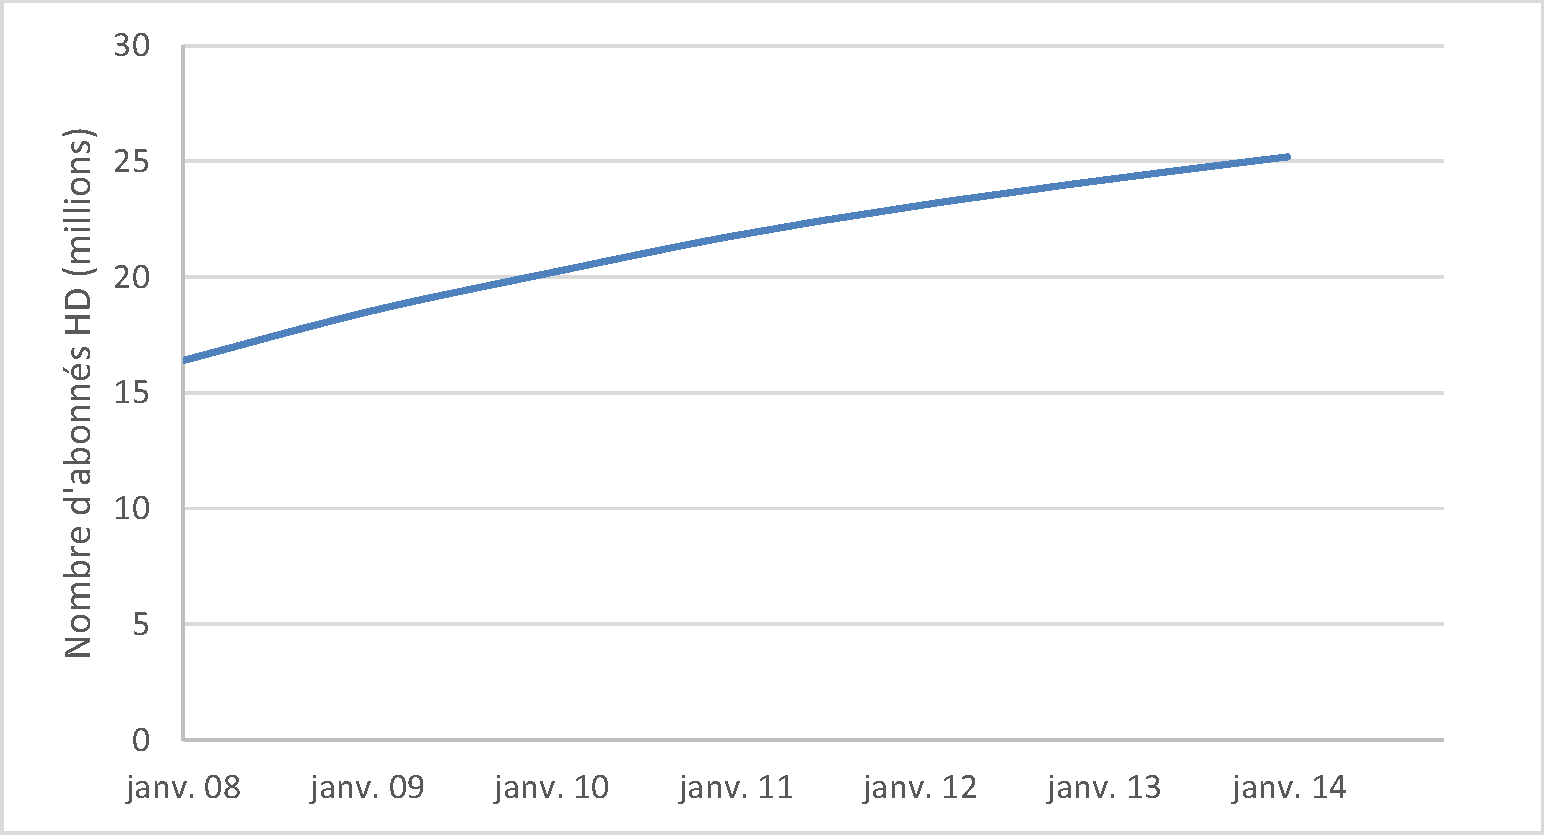
\includegraphics[width=0.9\linewidth]{img/abon_france}
\caption{Nombre d'abonnés à une offre Haut Débit en France}
\label{fig:abon_france}
\end{center}
\end{minipage}
\hfill
\begin{minipage}{0.4\linewidth}
Les FAI sont les seuls à pouvoir fournir un accès à internet pour les particuliers. \\ Depuis l'introduction de leurs services, le nombre d'abonnés aux offres de Haut Débit (HD) en France n'a pas cessé d'augmenter, comme le montre la courbe \ref{fig:abon_france} .
\end{minipage}
\end{figure}

\begin{figure}[htbp]
\begin{minipage}{0.45\linewidth}
Ce marché est géré par plusieurs acteurs que sont \begin{itemize}
\item Orange, \item Free, \item SFR, \item Bouygues, \item ...
\end{itemize}

La répartition des abonnés entre ces acteurs, au premier trimestre 2014, est présentée sur la figure \ref{fig:HD_cam}.
\end{minipage}
\hfill
\begin{minipage}{0.5\linewidth}
\begin{center}
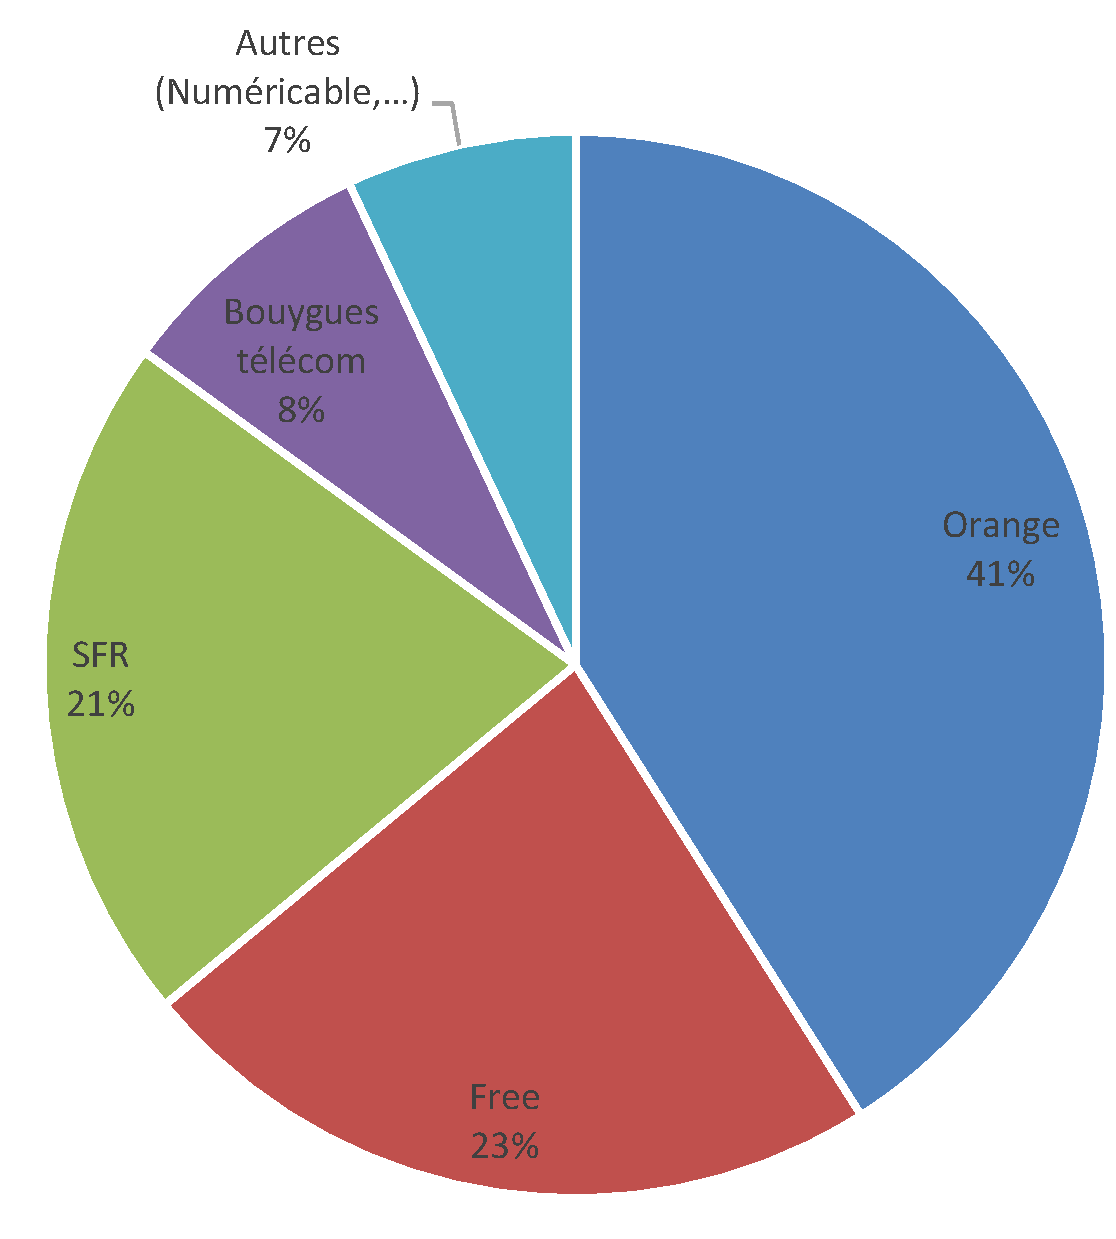
\includegraphics[width=0.7\linewidth]{img/HD_cam}
\caption{Répartition HD début 2014}
\label{fig:HD_cam}
\end{center}
\end{minipage}
\end{figure}

\paragraph{Question 1:} A partir de ces données, calculer le nombre d'abonnés Haut Débit chez l'opérateur Free au premier trimestre 2014 ?

~\

La figure \ref{fig:abon_free} donne l'évolution du nombre d'abonnés chez cet opérateur.

\begin{figure}[htbp]
\begin{center}
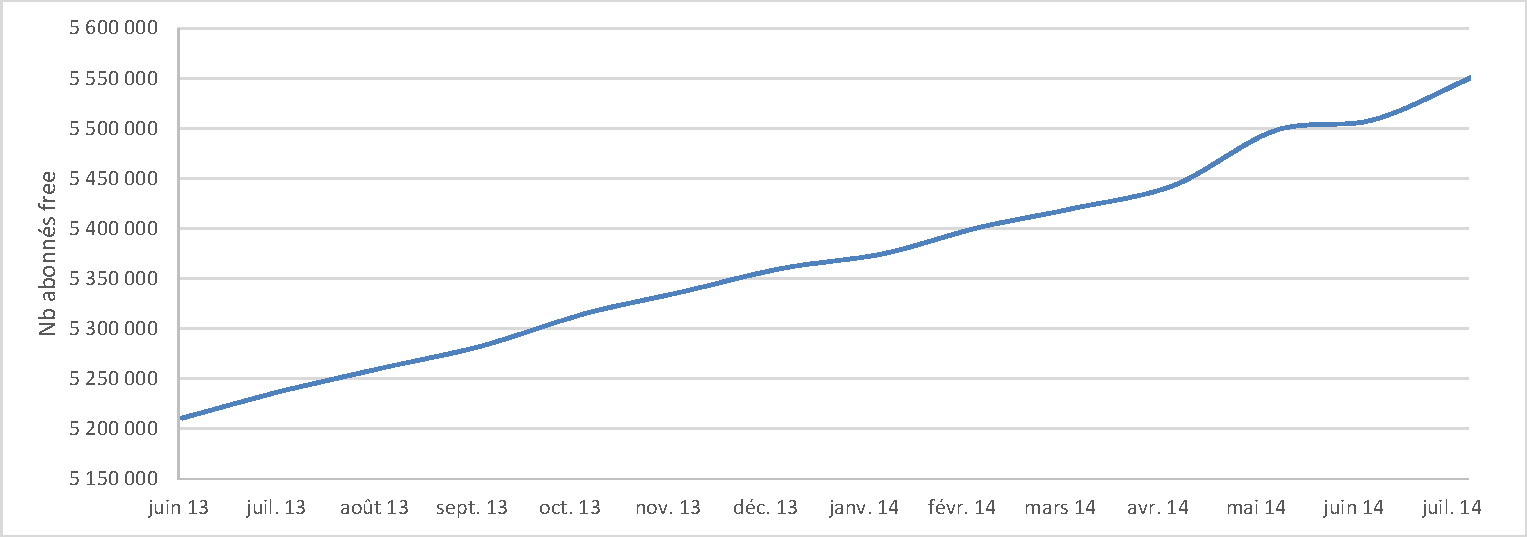
\includegraphics[width=0.8\linewidth]{img/abon_free}
\caption{Nombre d'abonnés Free}
\label{fig:abon_free}
\end{center}
\end{figure}

\paragraph{Question 2:} Cette figure vous permet-elle de valider le résultat de la question précédente.

\paragraph{Question 3:} Que pouvez-vous dire concernant cette évolution ?

\subsection{La stratégie de communication chez Free}

Vous disposez de captures de site web des principaux FAI en France:
\begin{itemize}
 \item \url{www.orange.fr/}
 \item \url{www.free.fr/}
 \item \url{www.sfr.fr/}
 \item \url{www.bouyguestelecom.fr/}
\end{itemize}

\paragraph{Question 4:} Après avoir consulté les sites web des différents FAI, vous donnerez pour chacun deux choix marketing qui ont été fait afin de convaincre les clients de choisir leur offre.

Notamment concernant les sujets suivants :
\begin{itemize}
 \item Le prix,
 \item Le service (vitesse,...),
 \item La garantie (grand réseau, service client,...),
 \item Le nombre d'abonnés,
 \item Les services en ligne (vidéo, abonnements tv, jeux,...),
 \item Le matériel (box, design, caractéristiques,...),
 \item Autres (téléphone,...)
 \item ...
\end{itemize}

Nous allons dans la suite nous intéresser au produit \og Freebox \fg qui fait partie des services proposés par l'opérateur Free.

\subsection{Présentation du produit}

\begin{figure}[htbp]
\begin{minipage}[c]{.35\linewidth}
\begin{center}
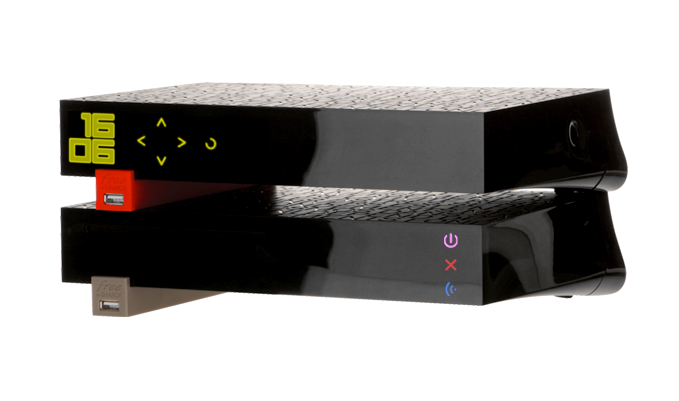
\includegraphics[width=\linewidth]{img/freebox.png}
\caption{Freebox}
\label{fig:image1}
\end{center}
\end{minipage}
\hfill
\begin{minipage}[c]{.62\linewidth}
La Freebox est un appareil électronique fourni par le fournisseur d'accès à Internet français Free à ses abonnés haut débit. La Freebox a connu six versions différentes depuis son premier lancement (avec des sous-versions apportant des changements plus ou moins importants). Elle se compose d'un boîtier permettant la connexion avec le réseau téléphonique et un second appareil permettant la diffusion de média sur divers éléments Hi-Fi (télévision, chaîne Stéréo,...).
\end{minipage}
\end{figure}

\subsection{Les services proposés par le produit}

\begin{figure}[htbp]
\begin{minipage}{0.65\linewidth}
Cet appareil sert principalement de modem ADSL ou FTTH, mais il est défini par la société Free comme \og un appareil électronique servant d'interface entre l'équipement informatique et/ou audiovisuel de l'usager et le réseau de Free \fg. En ce sens, il ne sert pas seulement d'interface entre un ordinateur et l'Internet, mais permet aussi à Free de proposer des services ajoutés utilisant le réseau, comme la télévision sur IP ou la téléphonie sur IP, trio que l'on connait sous l'appellation triple play. La Freebox peut également faire office de routeur et de point d'accès sans fil Wi-Fi. La Freebox est définie comme l'équipement terminal du réseau; elle demeure la propriété de Free, et n'est que prêtée aux abonnés. Elle est livrée avec une télécommande et des accessoires (câbles, filtre).
\end{minipage}
\hfill
\begin{minipage}[c]{.30\linewidth}
\begin{center}
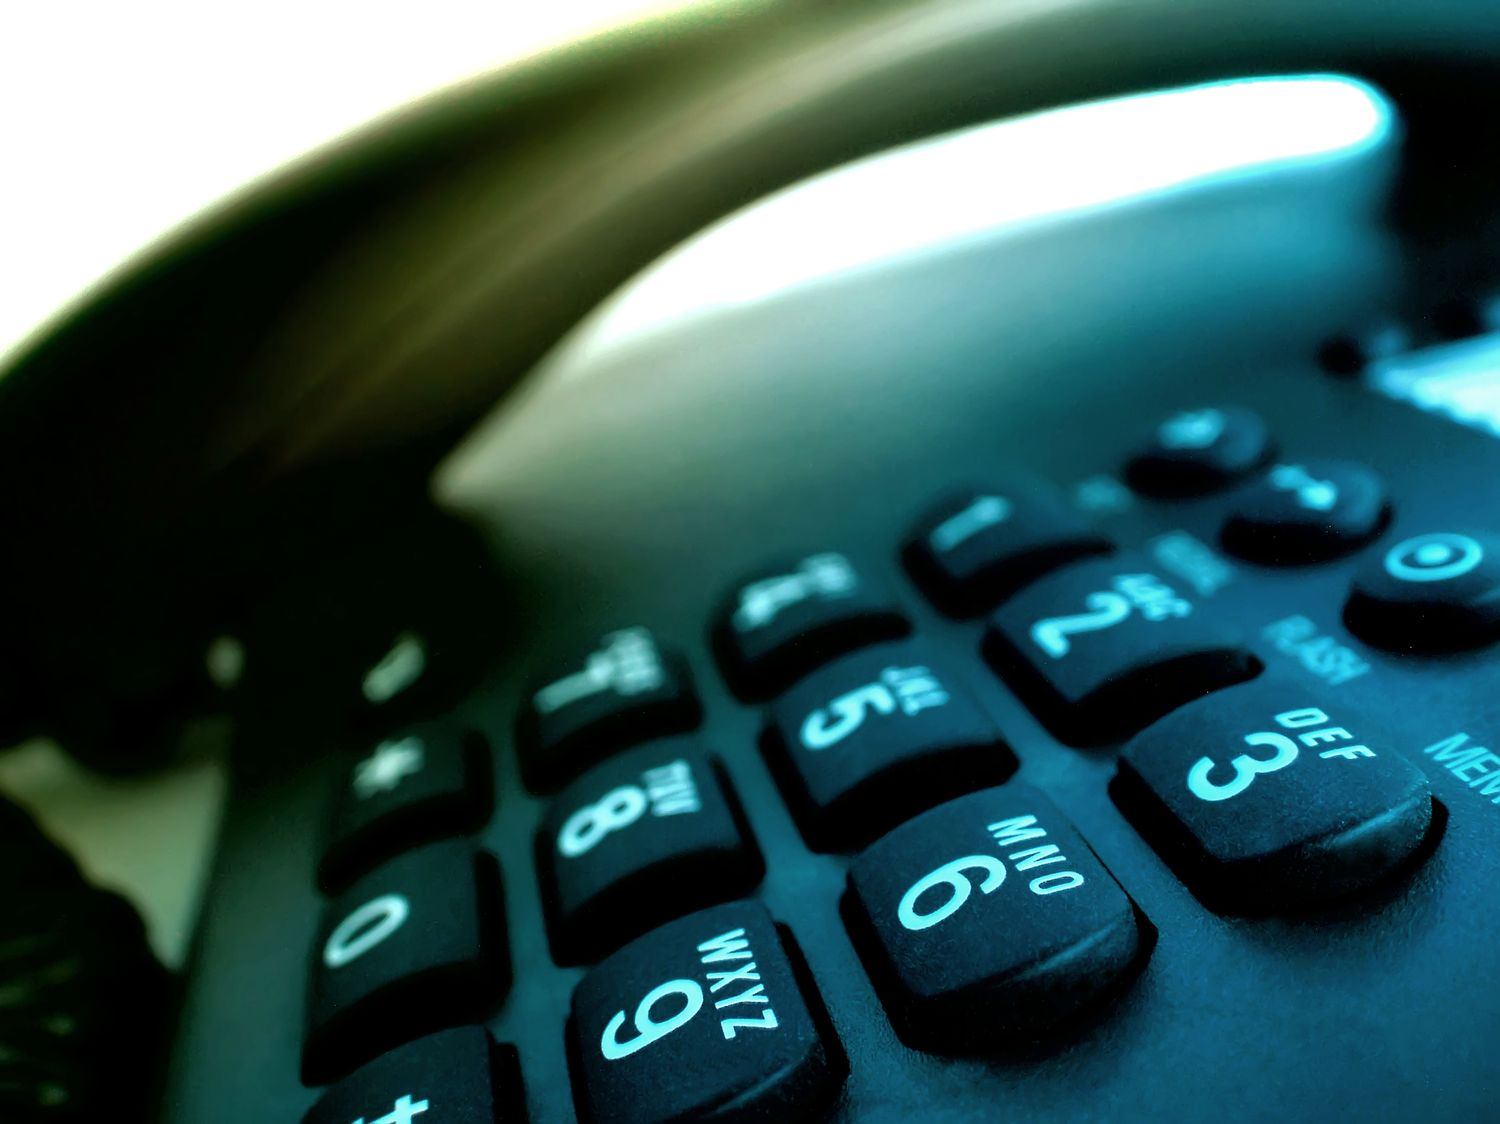
\includegraphics[width=\linewidth]{img/telephone.jpg}
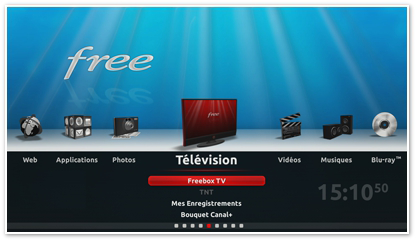
\includegraphics[width=\linewidth]{img/tv-free.png}
\caption{Télévision Free}
\label{fig:image2}
\end{center}
\end{minipage}
\end{figure}

\textit{Après avoir recherché dans le document de cours la définition d'un \og acteur \fg.}

\paragraph{Question 5:} Déterminer en justifiant quels sont le(s) acteur(s) principal(aux) et le(s) acteur(s) secondaire(s) de ce système.

~\

Sachant qui seront les acteurs liés à ce système, il est maintenant possible de déterminer sa fonction \og A quoi va-t-il servir ? \fg. Dans cette optique, la figure \ref{fig:image3} présente une partie des cas d'utilisation de la Freebox.

\begin{figure}[htbp]
\begin{center}
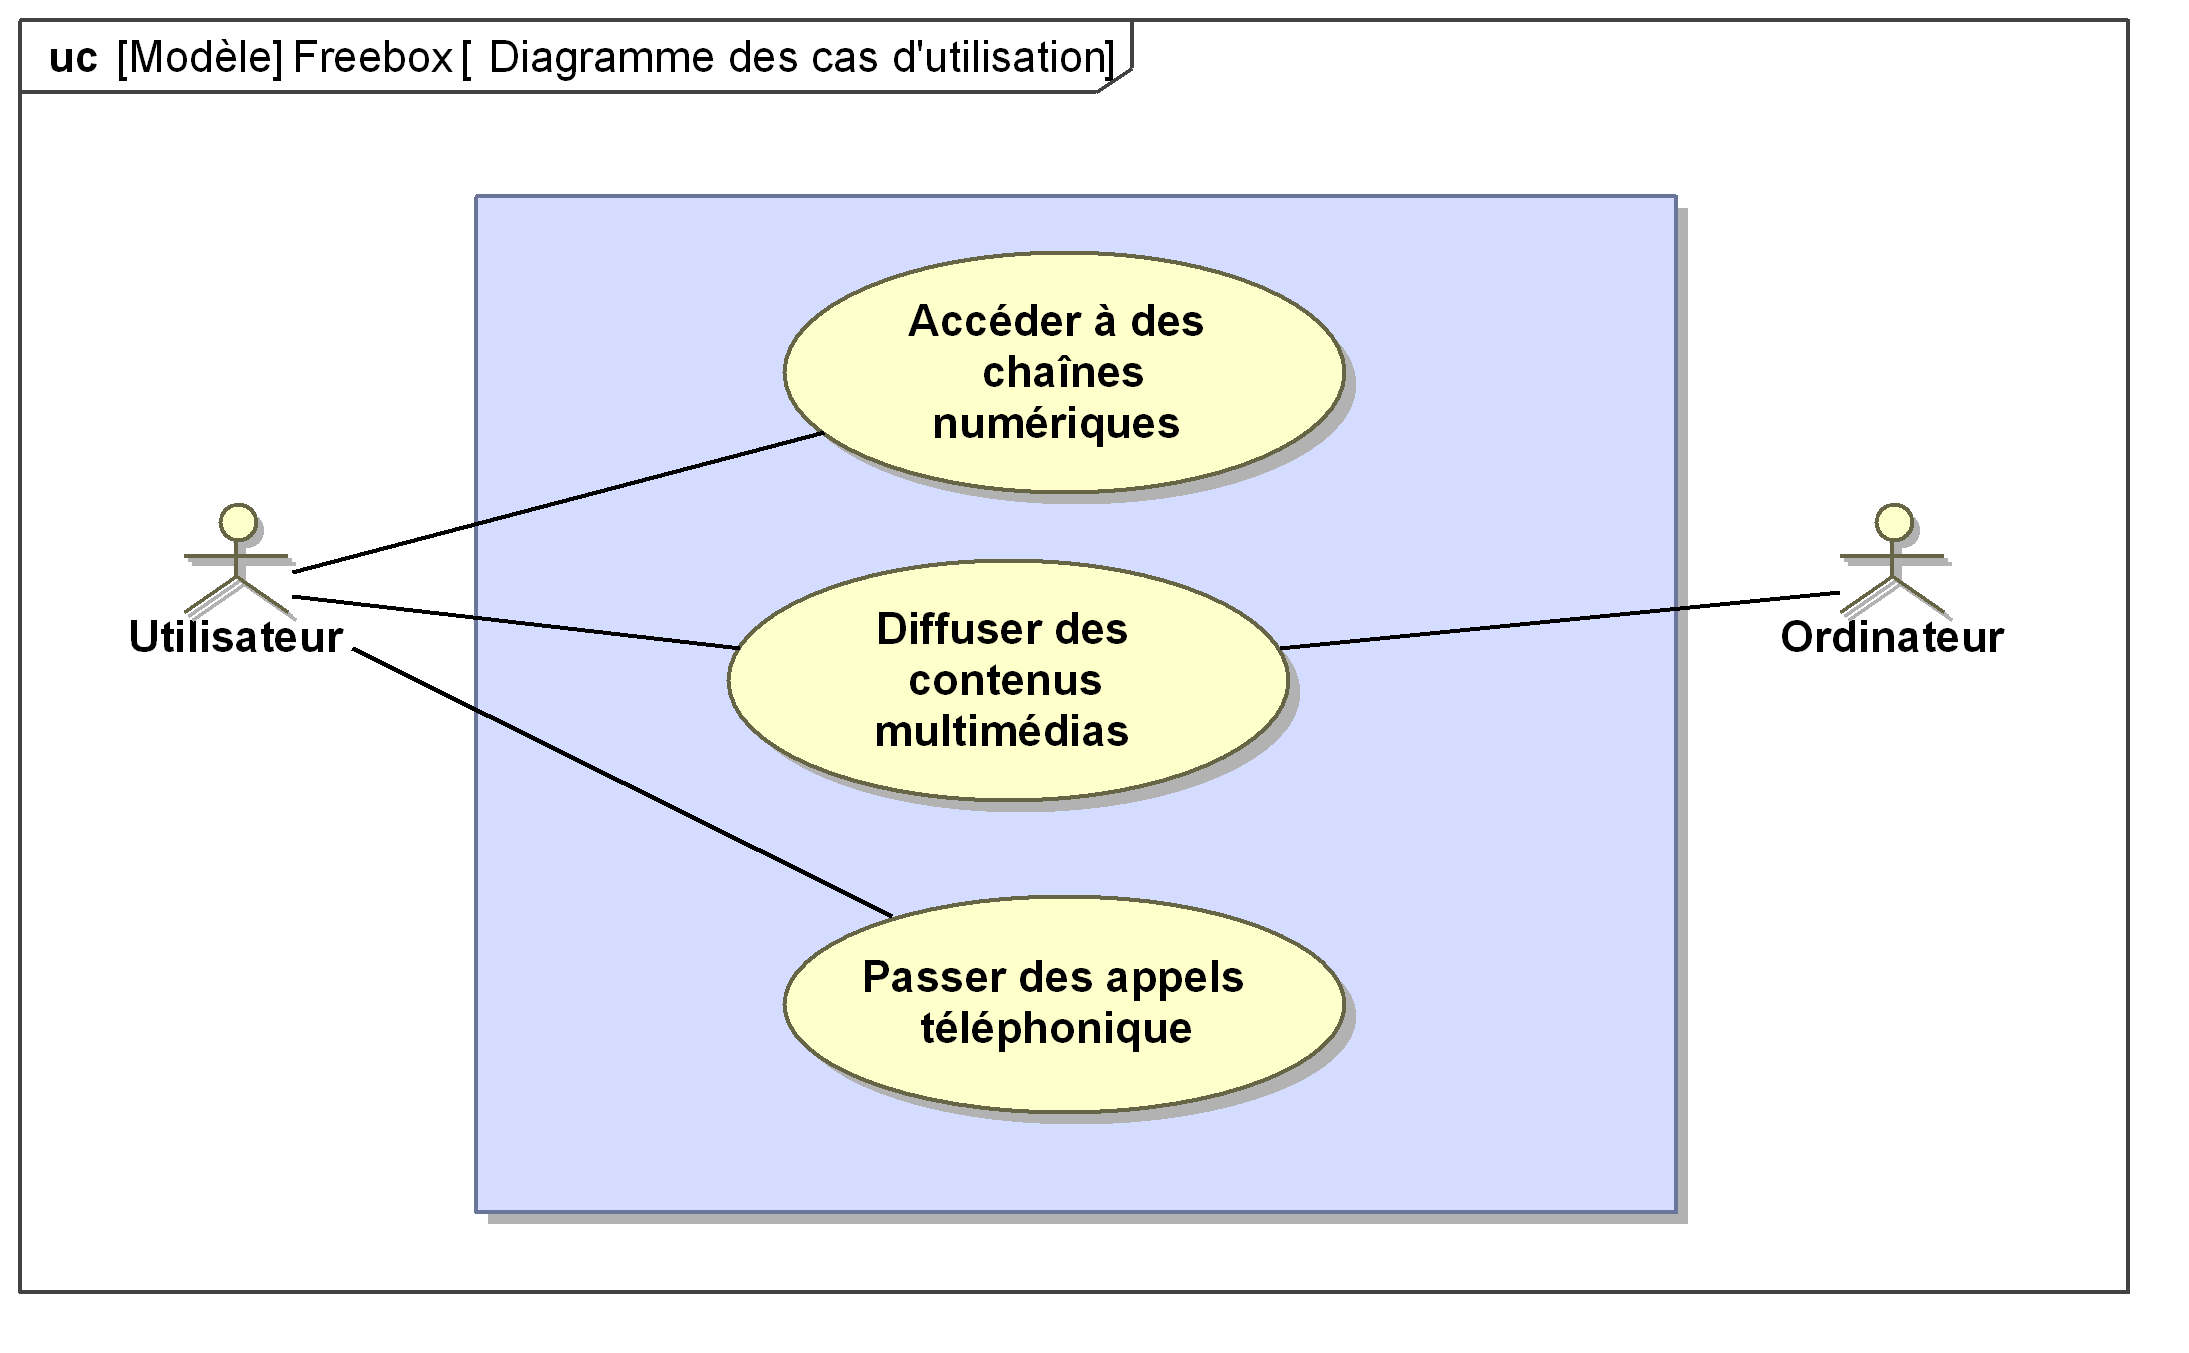
\includegraphics[width=0.8\linewidth]{img/Freebox_use_case}
\caption{Diagramme des Cas d'Utilisation}
\label{fig:image3}
\end{center}
\end{figure}

\textit{Après avoir recherché dans le document de cours la définition ainsi que les méthode de représentation d'un \og diagramme des cas d'utilisation \fg.}

\paragraph{Question 6:} En considérant les documents étudiés précédemment pensez-vous que ce diagramme soit complet ? Si cela est nécessaire, le compléter.

Des exigences ont-été issues du diagramme des cas d'utilisation précédent. Une partie de ces exigences sont présentées sur le diagramme des exigences de la figure \ref{fig:image38}. Certaines exigences du cahier des charges viennent des cas d'utilisation (implicites) d'autres sont imposées par diverses contraintes.

\textit{Après avoir recherché dans le document de cours la définition ainsi que les méthode de représentation d'un \og diagramme d'exigences \fg.}

\begin{figure}[!h]
\begin{center}
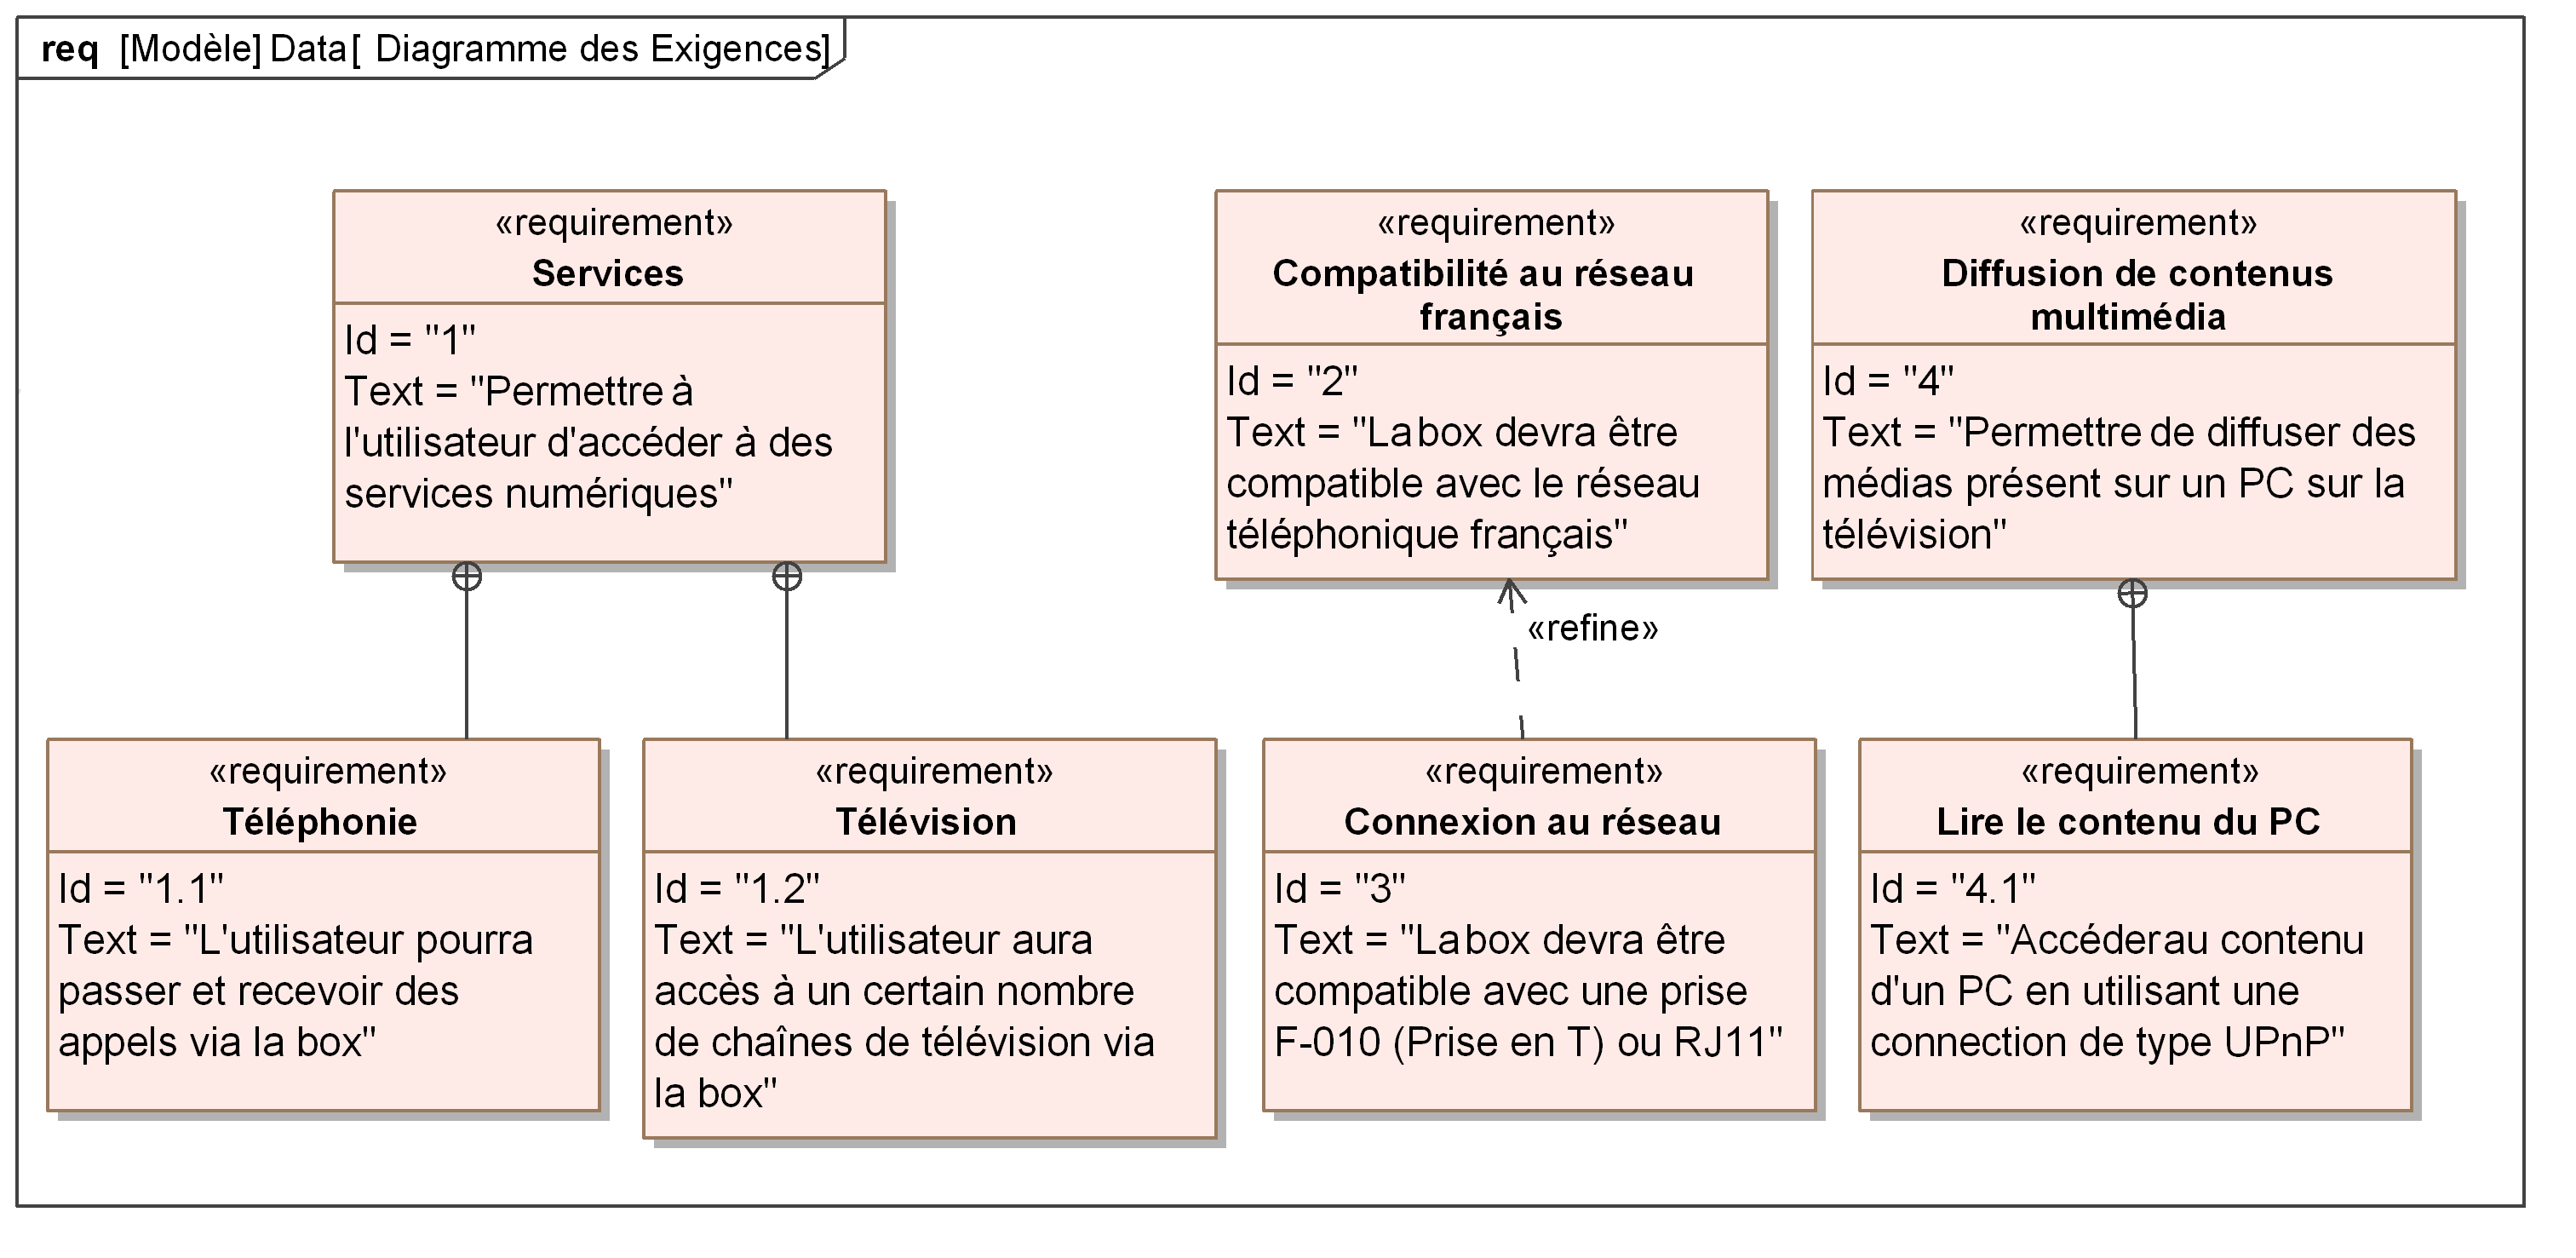
\includegraphics[width=0.9\linewidth]{img/Freebox_exigences}
\caption{Diagramme des Exigences}
\label{fig:image38}
\end{center}
\end{figure}


\paragraph{Question 7:} Compléter le diagramme des exigences en prenant en compte les cas d'utilisation que vous avez ajouté. Chaque exigence que vous ajouterez devra être décomposée en deux sous-exigences.

\paragraph{Question 8:} Retrouvez ensuite, à chaque fois que c'est possible à quel cas d'utilisation correspond chaque exigence.

\paragraph{Question 9:} Vous donnerez à chacune des exigences présentes sur ce diagramme une note qui caractériser sont niveau (1:Indispensable, 2: Très importante, 3: Importante, 4:Peu importante)

\subsection{Les acteurs du système}

Une fois le Besoin clairement identifié, il est nécessaire de préciser l'ensemble des Éléments du Milieu Environnant/Extérieur (EME) qui interagissent avec le produit. Ainsi, la totalité des Fonctions de Service que devra remplir le produit pour garantir un bon fonctionnement dans toutes les conditions d'utilisation pourront être déterminées.

\textit{Après avoir recherché dans le document de cours la définition d'une \og phase de vie \fg.}

\paragraph{Question 10:} Énumérez les phases de vie du système Freebox.

\begin{figure}[!h]
\begin{center}
\begin{tabular}{|c|c|c|}
\hline
........................ & ........................ & ........................ \\
\hline
........................ & ........................ & ........................ \\
\hline
........................ & ........................ & ........................ \\
\hline
........................ & ........................ & ........................ \\
\hline
\end{tabular}
\end{center}
\caption{Liste des phases de vie}
\end{figure}

\paragraph{\textit{Données supplémentaires}}

Le diagramme de contexte de la figure \ref{fig:image35} introduit les éléments du milieu extérieur au système.

\begin{figure}[!h]
\begin{center}
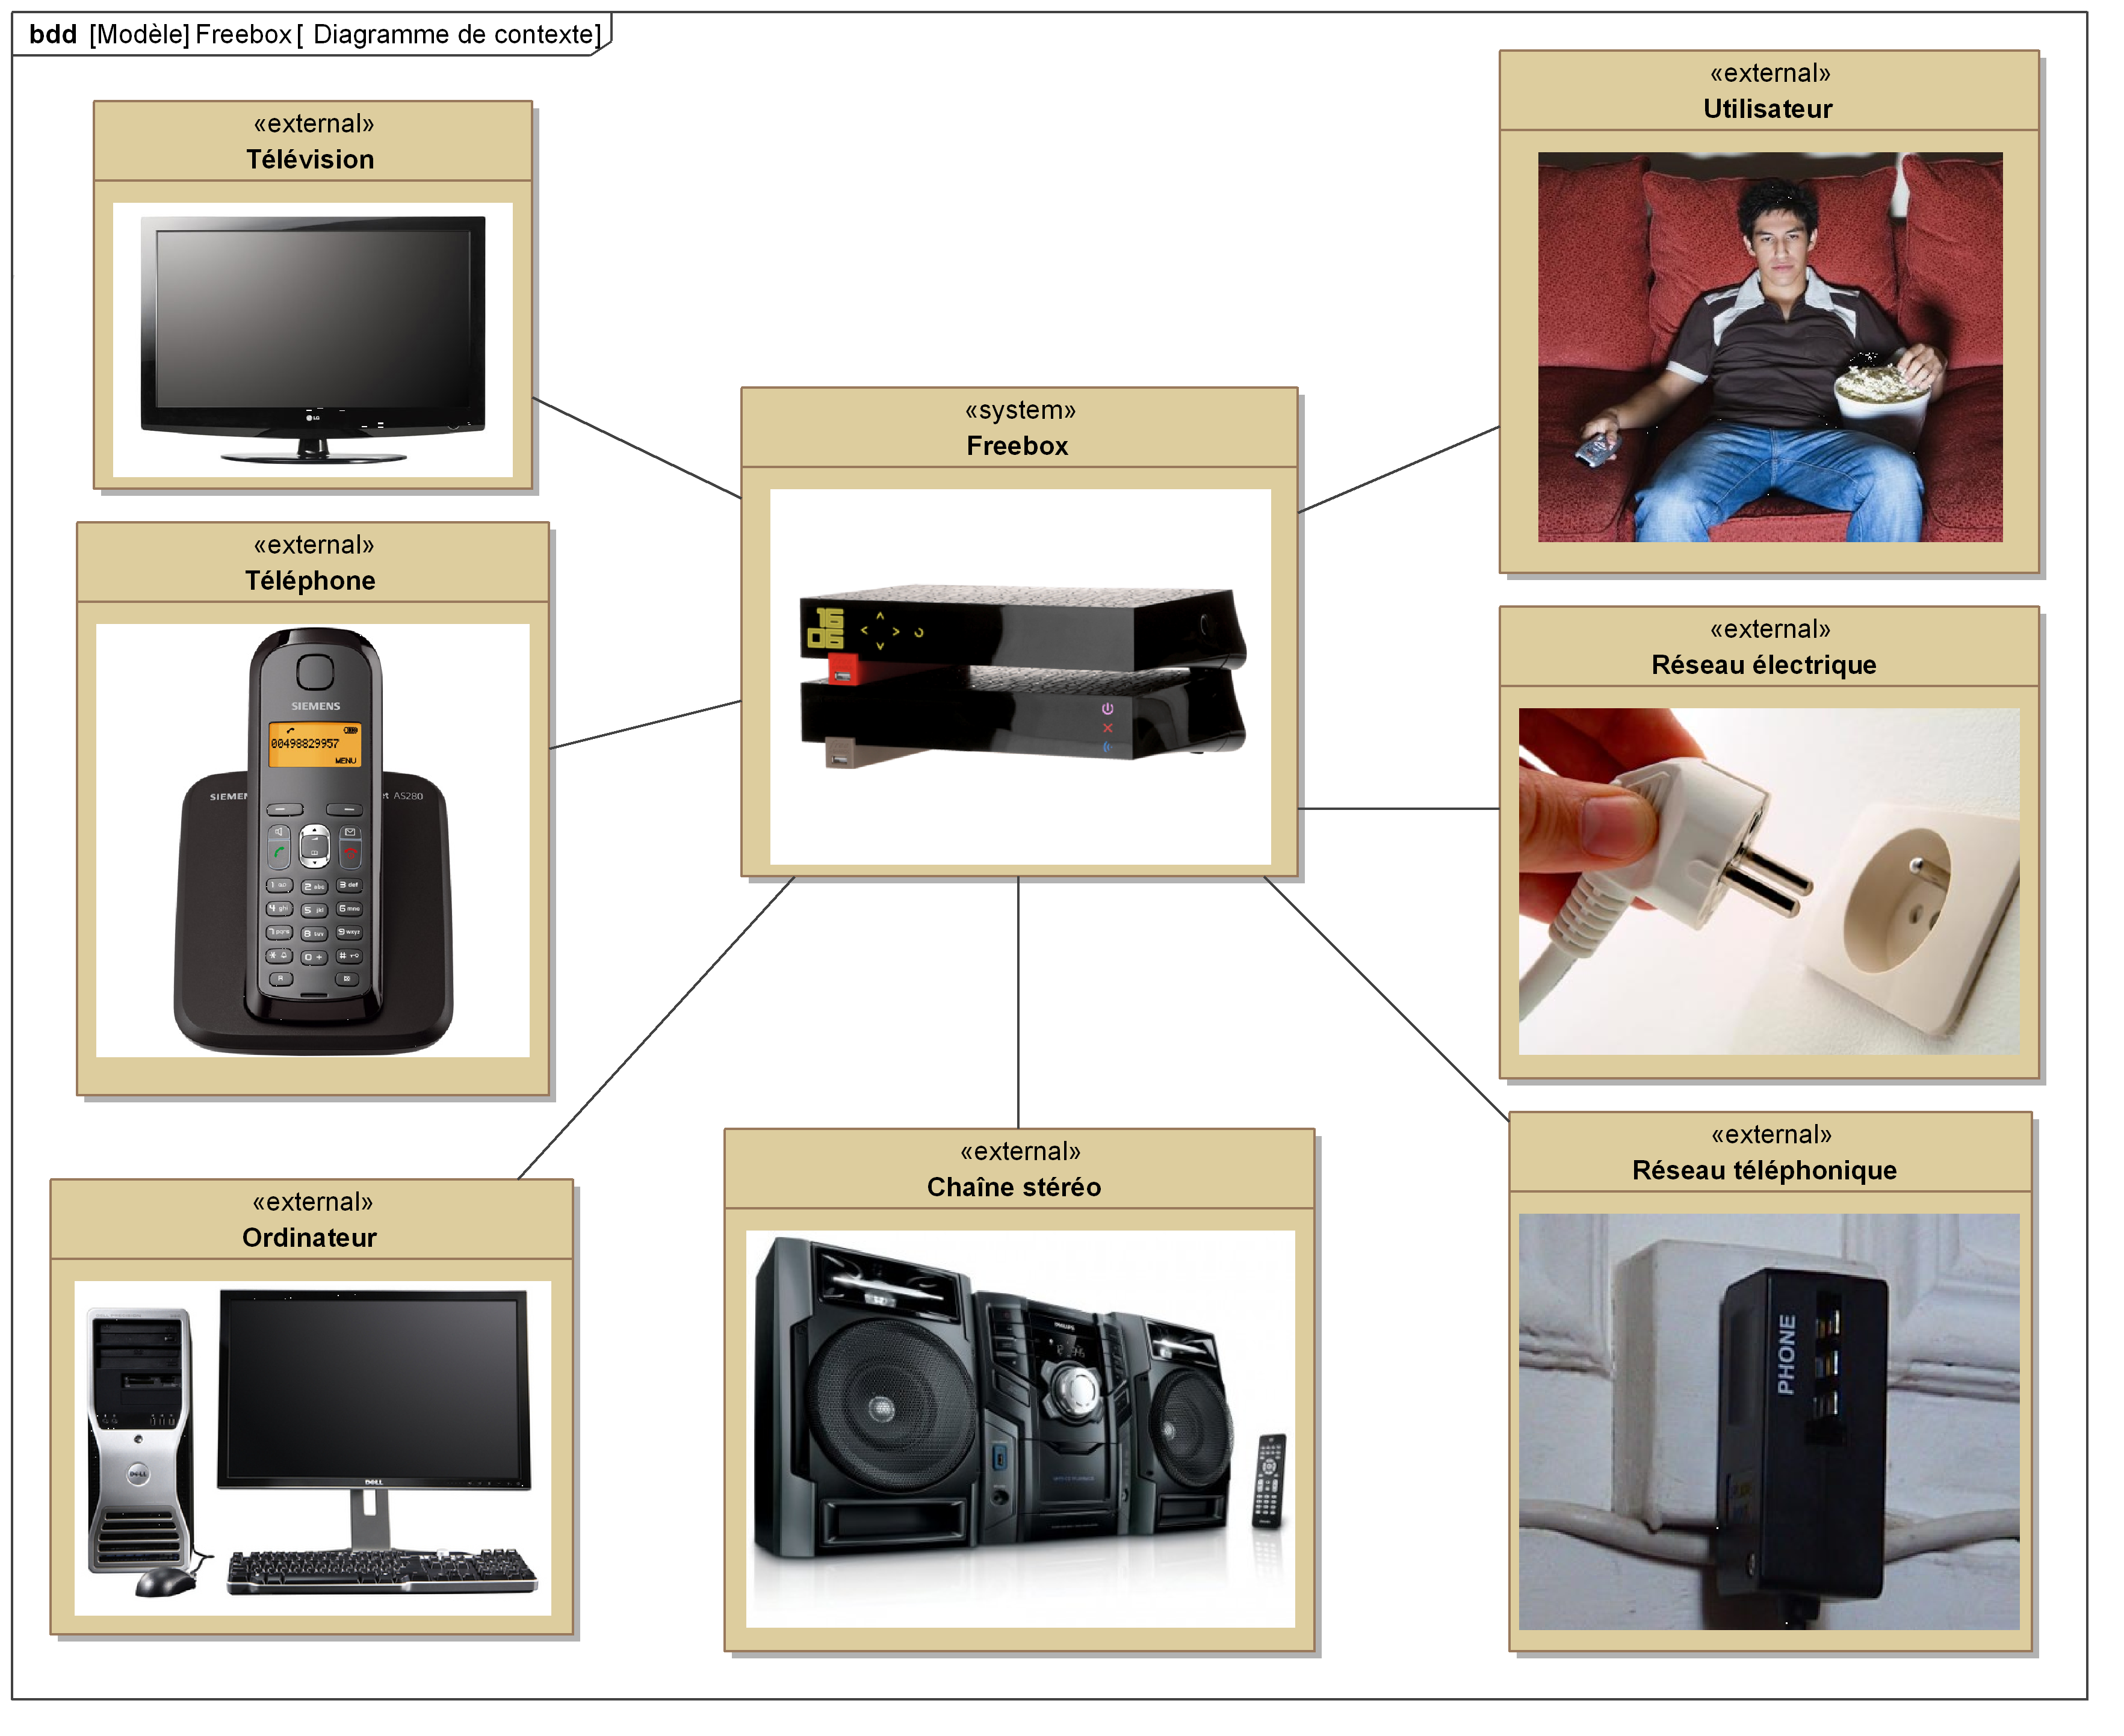
\includegraphics[width=0.7\linewidth]{img/Freebox_contexte}
\caption{Diagramme de Contexte}
\label{fig:image35}
\end{center}
\end{figure}

Description des Éléments du Milieu Environnant:

\begin{figure}[!h]
\begin{center}
\begin{tabular}{|c|c|}
\hline
\textbf{Éléments} & \begin{tabular}{c} \textbf{Description et hypothèse sur toutes} \\ \textbf{les caractéristiques de l'élément} \end{tabular} \\
\hline
Réseau électrique & \begin{tabular}{c} Source d'énergie classique, disponible dans une habitation, \\ soit énergie électrique de nature EDF (220v 50 Hz) \end{tabular} \\
\hline
\begin{tabular}{c} Réseau téléphonique \\ (et internet) \end{tabular} & \begin{tabular}{c} Réseau téléphonique classique, adaptateur pour \\ une prise F-010 (prise en T, norme CEI 60603-7 (RJ45)) \end{tabular} \\
\hline
Utilisateur &  \begin{tabular}{c} Toute personne en âge de faire \\ fonctionner ces appareils (7 ans) \end{tabular} \\
\hline
Télévision & \begin{tabular}{c} Poste équipé de prises \\ HDMI et péritel \end{tabular} \\
\hline
Téléphone & \begin{tabular}{c} Téléphone à connecteur sur \\ le réseau téléphonique classique \end{tabular} \\
\hline
Ordinateur & \begin{tabular}{c} Ordinateur possédant une carte réseau \\ (Wi-Fi et/ou RJ45) + logiciels \end{tabular} \\
\hline
Chaîne Stéréo & \begin{tabular}{c} Chaîne stéréo possédant des connections \\ RCA, jack et/ou numérique \end{tabular} \\
\hline
\end{tabular}
\end{center}
\caption{Liste des Éléments du Milieu Extérieur}
\end{figure}

Les éléments qui apparaissent dans un diagramme de contexte ne sont pas forcément tous nécessaires au fonctionnement du système.

\paragraph{Question 11:} Donner l'ensemble des éléments extérieurs nécessaires au bon fonctionnement de la freebox.

\paragraph{Question 12:} Donner l'ensemble des éléments capable de \og constater \fg le fonctionnement du système. Ce sont les acteurs du système. Votre réponse correspond-elle au diagramme des cas d'utilisation de la figure \ref{fig:image3} ?

\subsection{Étude détaillée d'un cas d'utilisation}

\begin{figure}[!h]
\begin{minipage}{0.58\linewidth}
Un des cas d'utilisation du système était: \og Diffuser des contenus multimédias \fg. Ce cas d'utilisation correspond à une séquence d'échange entre plusieurs acteurs dont une description est faite à la figure \ref{fig:image4}.
\end{minipage}
\hfill
\begin{minipage}{0.4\linewidth}
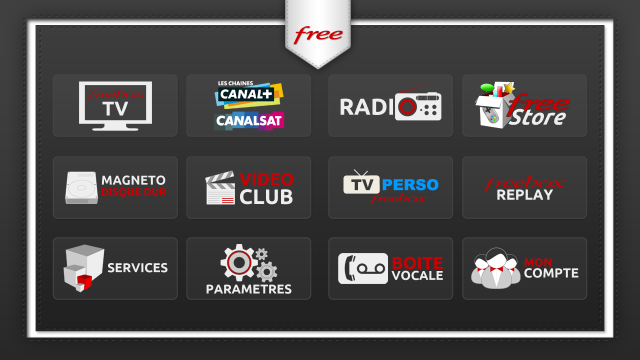
\includegraphics[width=0.8\linewidth]{img/menu}
\end{minipage}
\end{figure}

\begin{figure}[!h]
\begin{center}
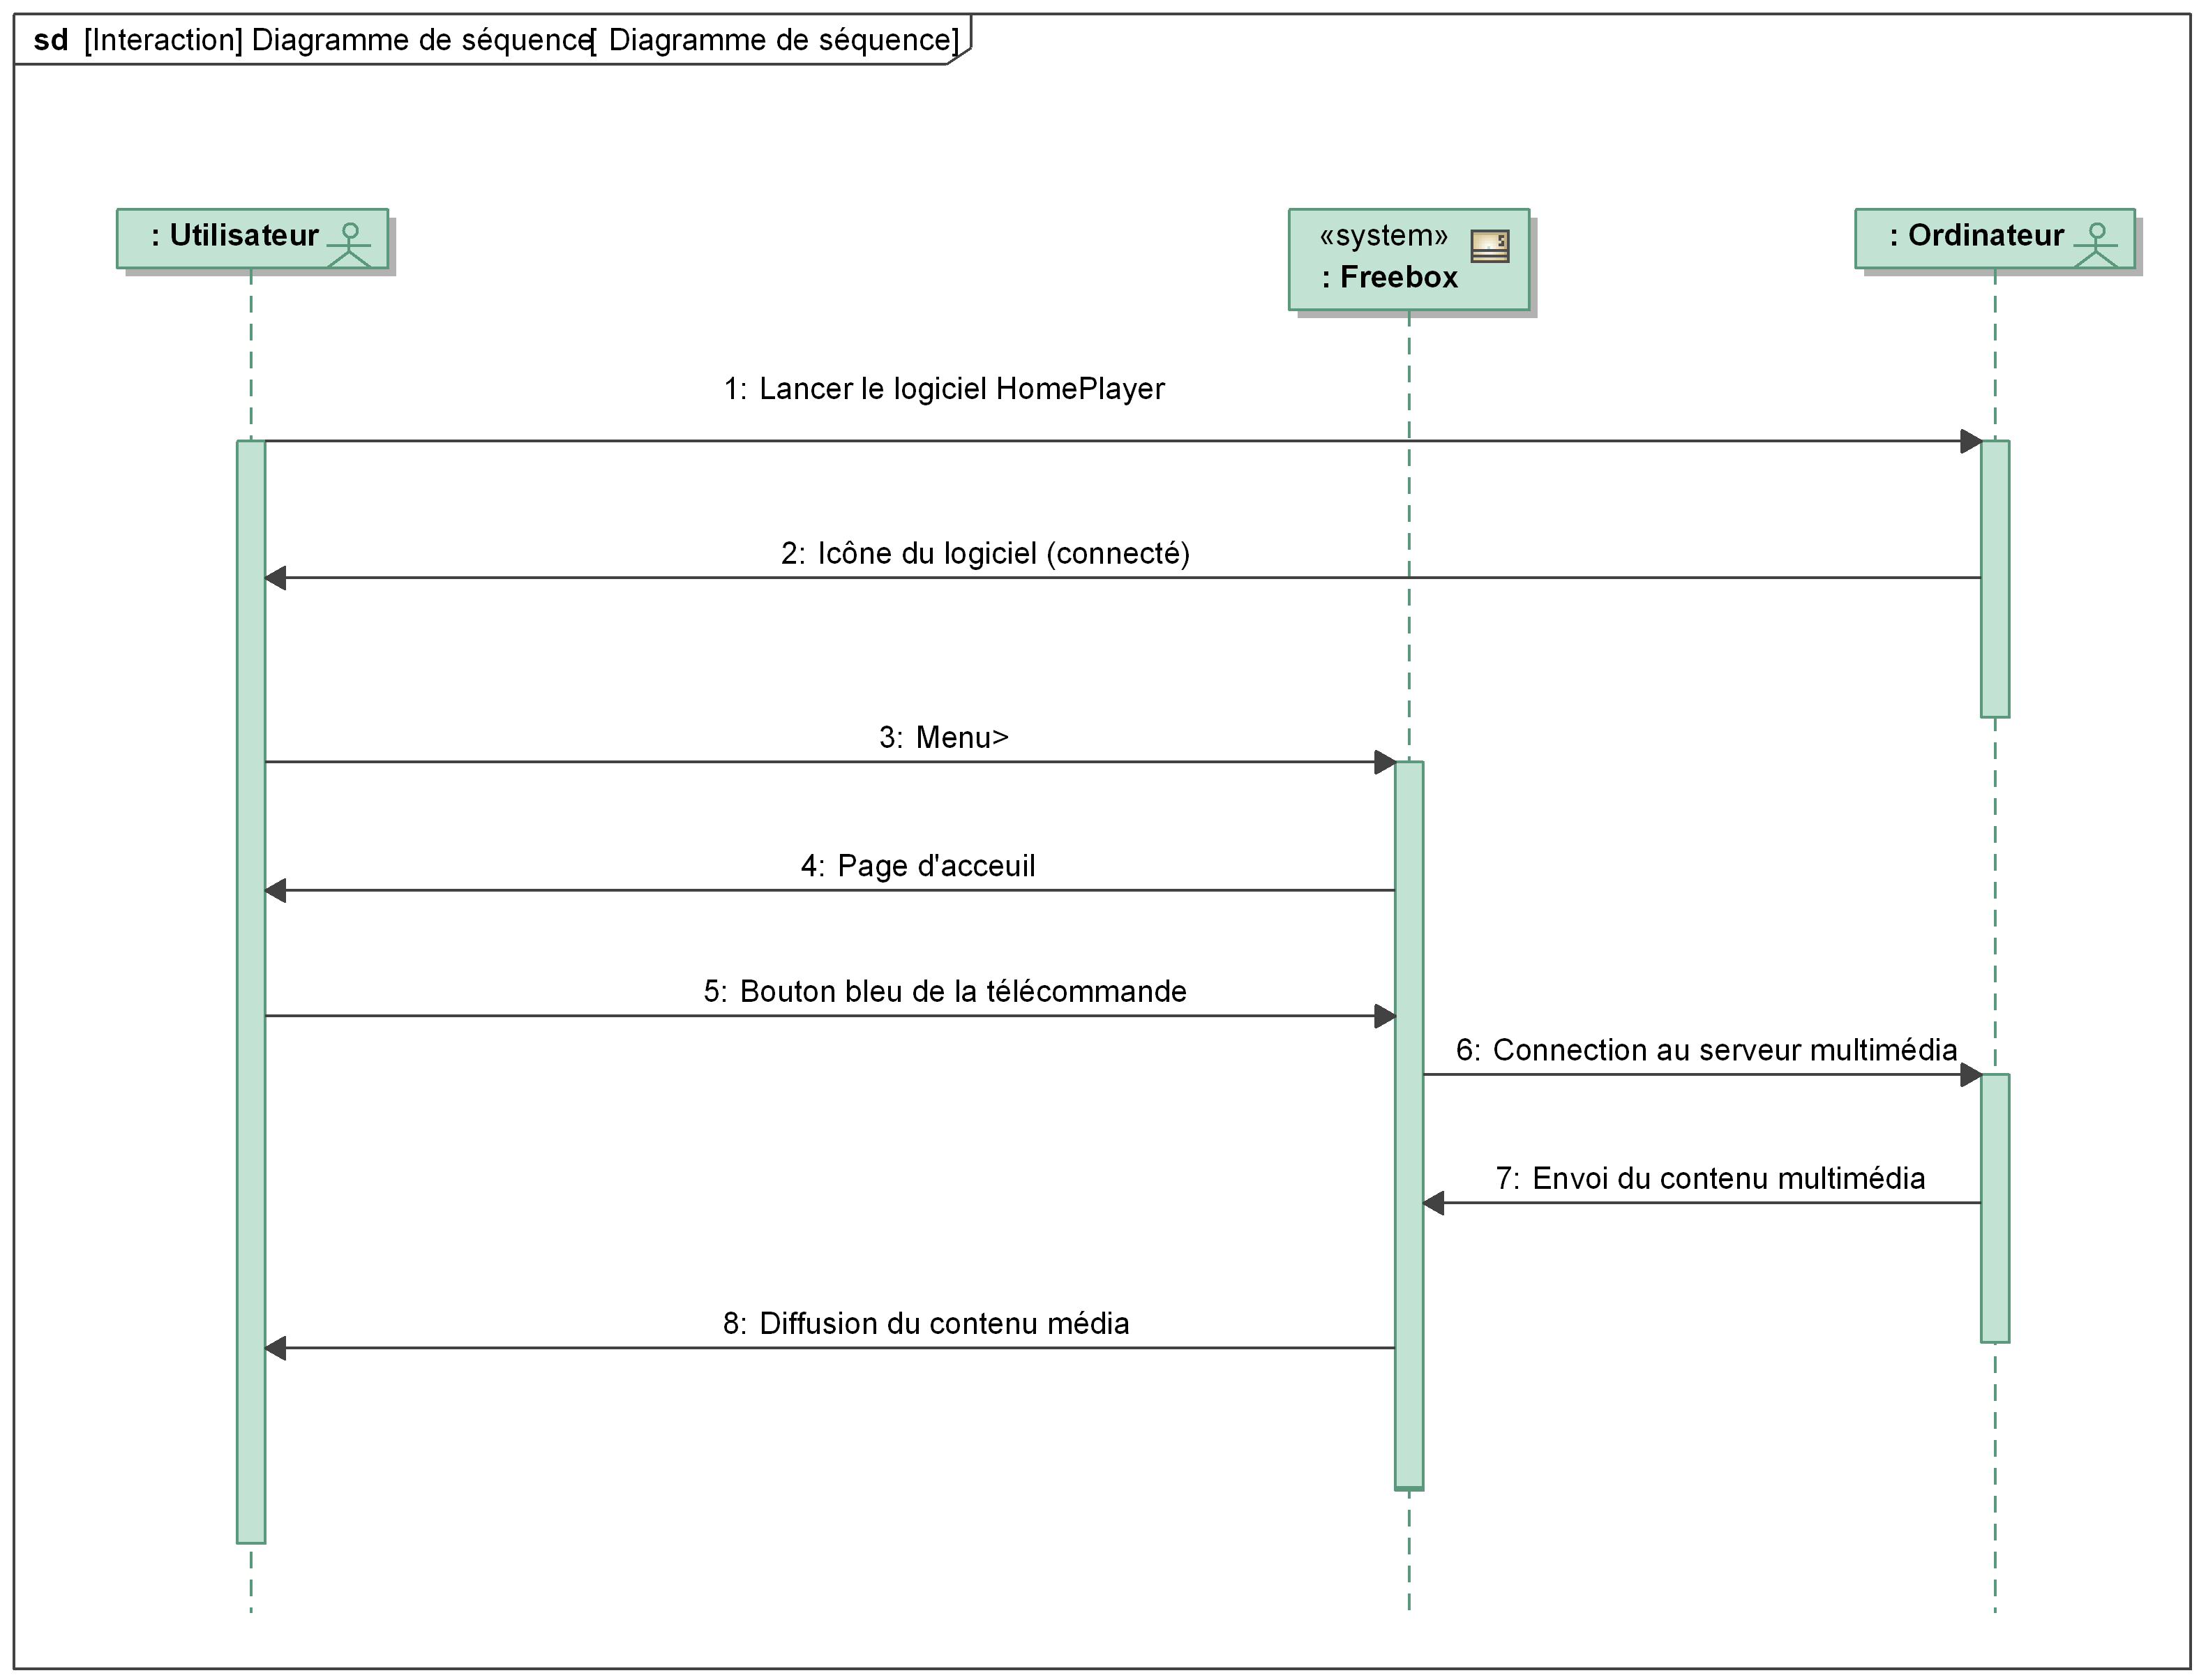
\includegraphics[width=0.9\linewidth]{img/Freebox_sequence}
\caption{Diagramme de Séquence}
\label{fig:image4}
\end{center}
\end{figure}

\paragraph{Question 13:} D'après la figue \ref{fig:image4} quels sont le ou les acteur(s) impliqué(s) dans cette séquence ? Quels sont les éléments du milieu extérieur concernés ? Cela correspond-il à ce qui est indiqué sur le diagramme des cas d'utilisation de la figure \ref{fig:image3} ?

Nous allons nous placer du point de vue de l'utilisateur pour répondre à la question suivante.

Il souhaite regarder une vidéo présente sur son PC et suit la séquence indiquée à la figure \ref{fig:image4}. La séquence se déroule normalement, cependant, lorsque l'utilisateur presse le bouton bleu à l'étape 5, même en attendant un long moment, la diffusion du contenu média n'arrive pas.

\paragraph{Question 14:} Quel est le composant le plus susceptible de ne pas fonctionner ? Fait-il partie du système ?

\newpage

\section{Étude d'une entreprise: Tembec Tartas S.A.}

\begin{figure}[htbp]
\begin{minipage}{0.43\linewidth}
\begin{center}
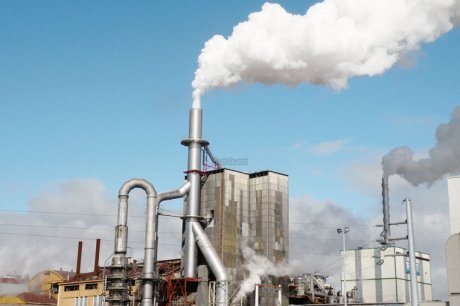
\includegraphics[width=\linewidth]{img/tartas.jpg}
\caption{Bioraffinerie}
\label{fig:tartas1}
\end{center}
\end{minipage}
\hfill
\begin{minipage}{0.46\linewidth}
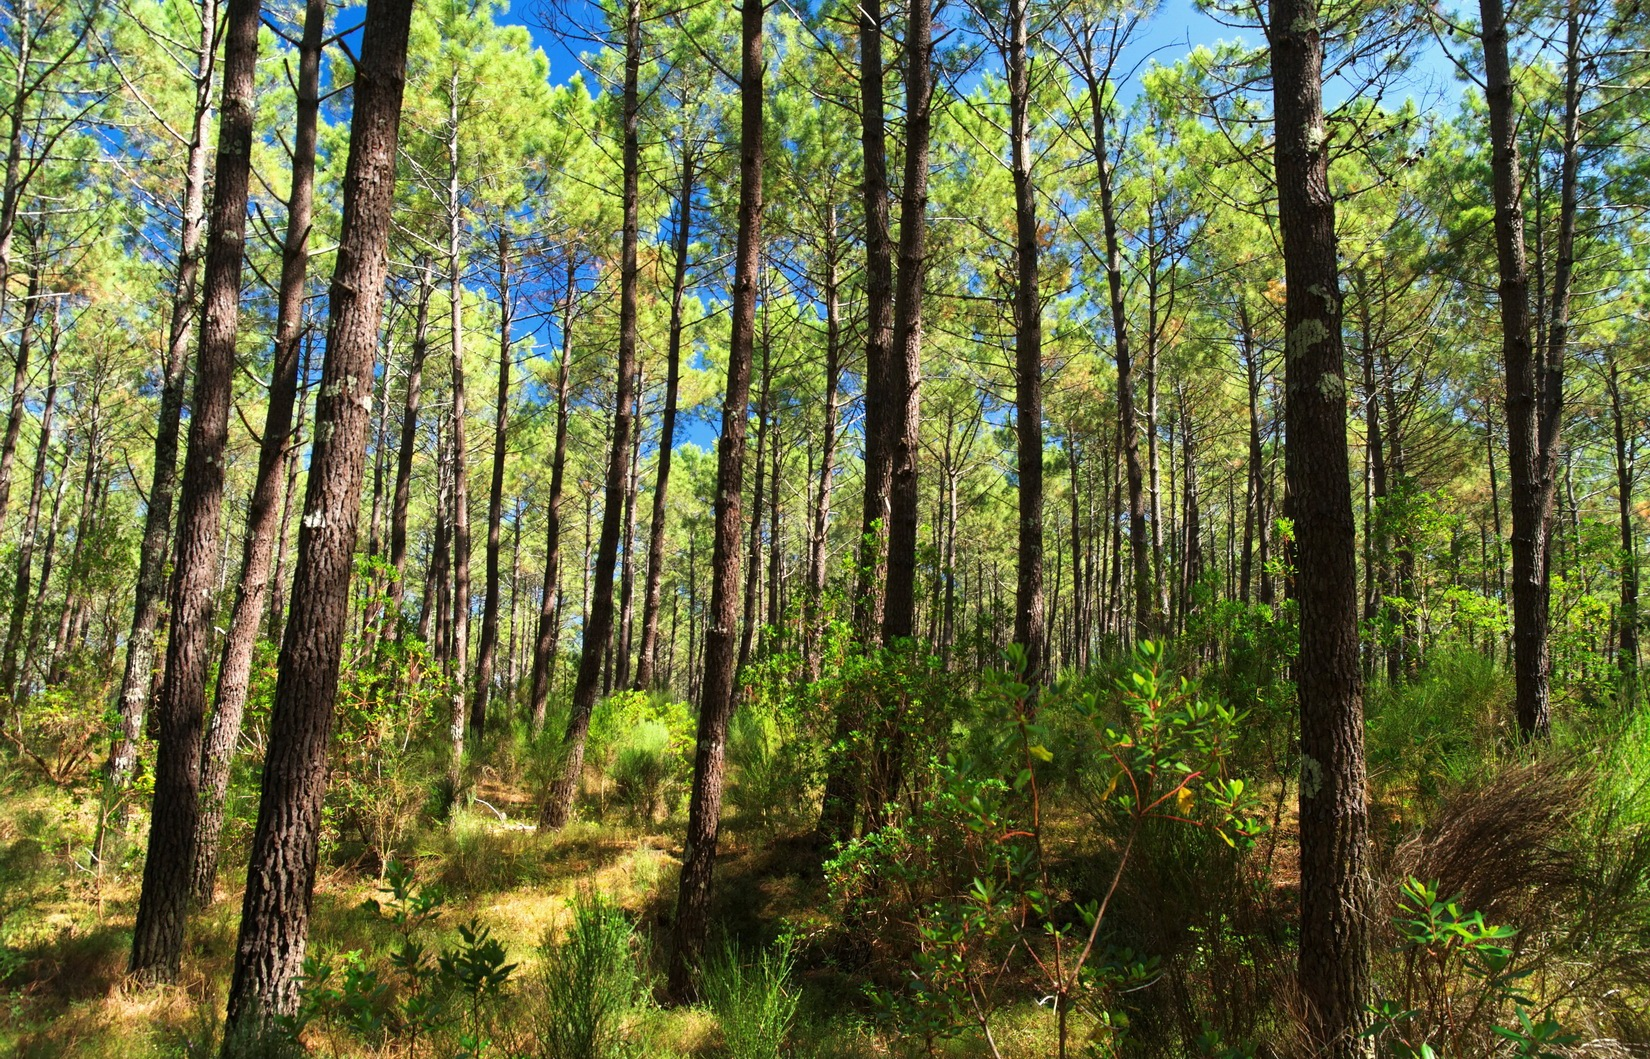
\includegraphics[width=\linewidth]{img/Pins.jpg}
\caption{Pins des landes}
\label{fig:tartas2}
\end{minipage}
\end{figure}

\subsection{Introduction}

\begin{figure}[htbp]
\begin{minipage}{0.55\linewidth}

Le bois est constitué principalement de matières organiques (cellulose et lignine) et d'un faible pourcentage (de 1 à 1,5 \%) d'éléments minéraux. Il contient également une part d'humidité variable.

Les proportions sont les suivantes:
\begin{itemize}
 \item Cellulose (environ 50 \%)
 \item Lignine (20 à 30 \%)
 \item Hémicellulose (15 à 25 \%) 
 \item Autres substances organiques : polysaccharides, pentosanes, hexosanes, résines, tannins, colorants, cires, alcaloïdes, etc.
\end{itemize}

\end{minipage}
\hfill
\begin{minipage}{0.35\linewidth}
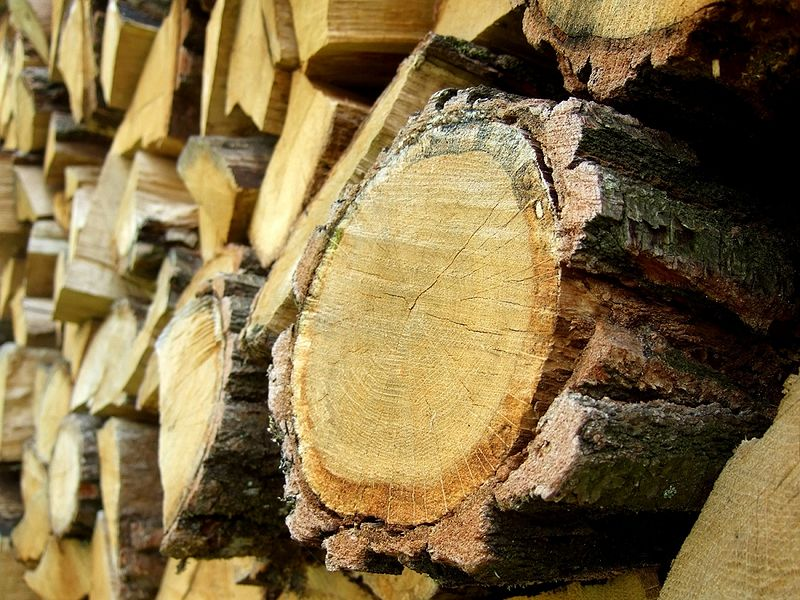
\includegraphics[width=\linewidth]{img/bois.jpg}
\caption{Bois: matière première}
\label{fig:tartas3}
\end{minipage}
\end{figure}

\subsection{Présentation de l'entreprise}

Le site de Tembec Tartas est une Bioraffinerie. Il s'agit d'une installation permettant de valoriser l'ensemble des composants des végétaux grâce à une bioconversion naturelle qui ne laisse aucun déchets.

Son objectif est d'extraire la cellulose de haute qualité contenue dans le pin maritime. Ce site landais est leader mondial dans les domaines les plus variés : épaississants et gélifiants pour l'alimentaire, pelliculage de comprimés pour la pharmacie, fluidité des crèmes pour les cosmétiques, vernis, peintures.

Le produit d'entrée est du bois. Celui-ci est transformé en suivant plusieurs étapes comme indiquées dans la figure \ref{fig:processus} en utilisant plusieurs moyens dont certains sont présentés sur la figure \ref{fig:tartas5}. Tous les co-produits (produits issus de la récupération de la cellulose) sont récupérés au fur et à mesure de la production et peuvent être utilisés (liqueur noire, lignine,...). Une partie de l'énergie consommée par la production vient de la combustion, dans des chaudières, de certains produits issus de la production. Cette entreprise est soumise à des exigences anti-pollution (sonore, olfactives, chimiques, énergétiques,...) très exigeantes qui constituent un objectif très important pour la production.

\begin{figure}[htbp]
	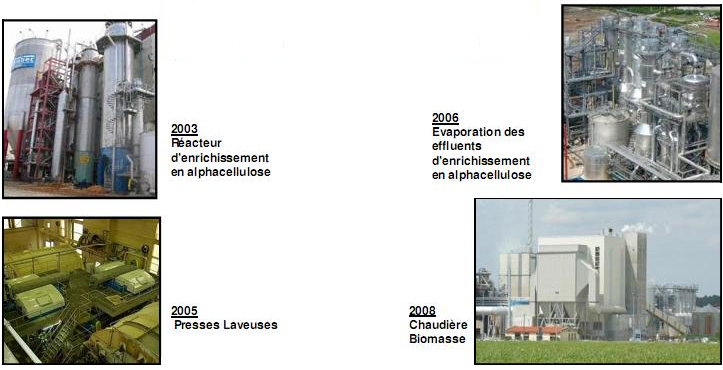
\includegraphics[width=\linewidth]{img/moyens.png}
	\caption{Moyens de l'entreprise}
	\label{fig:tartas5}
\end{figure}

\subsection{Présentation du produit}


\begin{figure}[htbp]
\begin{minipage}{0.55\linewidth}
Le produit principal, présenté figure \ref{fig:tartas6}, issu de ce processus de fabrication est une cellulose de haute qualité. La cellulose est le composant principal du papier mais peut être utilisé dans beaucoup d'applications, comme dans le bâtiment (peinture, colle, plâtre,...), dans l'agroalimentaire (additifs, ils portent les codes de E460 à E466) ainsi que dans d'autres domaines comme la fabrication d'explosifs...
\end{minipage}
\hfill
\begin{minipage}{0.48\linewidth}
\begin{center}
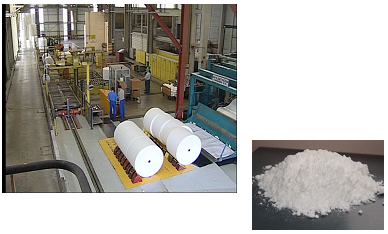
\includegraphics[width=0.7\linewidth]{img/produits.png}
\caption{Celluloses de spécialité}
\label{fig:tartas6}
\end{center}
\end{minipage}
\end{figure}

\subsection{Étude de l'entreprise}

La suite va porter sur l'étude de l'entreprise qui fabrique ce produit. Nous allons effectuer ce travail à l'aide des outils à notre disposition pour la mise en place d'une analyse fonctionnelle.

\paragraph{Question 1:}

Donner la liste des intéracteurs en contact avec cette entreprise. Vous mettrez ensuite cette liste sous la forme d'un diagramme de contexte.

Le diagramme des exigences de la figure \ref{fig:tartas_ex} présente un extrait du cahier des charges de l'entreprise. 

\begin{figure}[!h]
\begin{center}
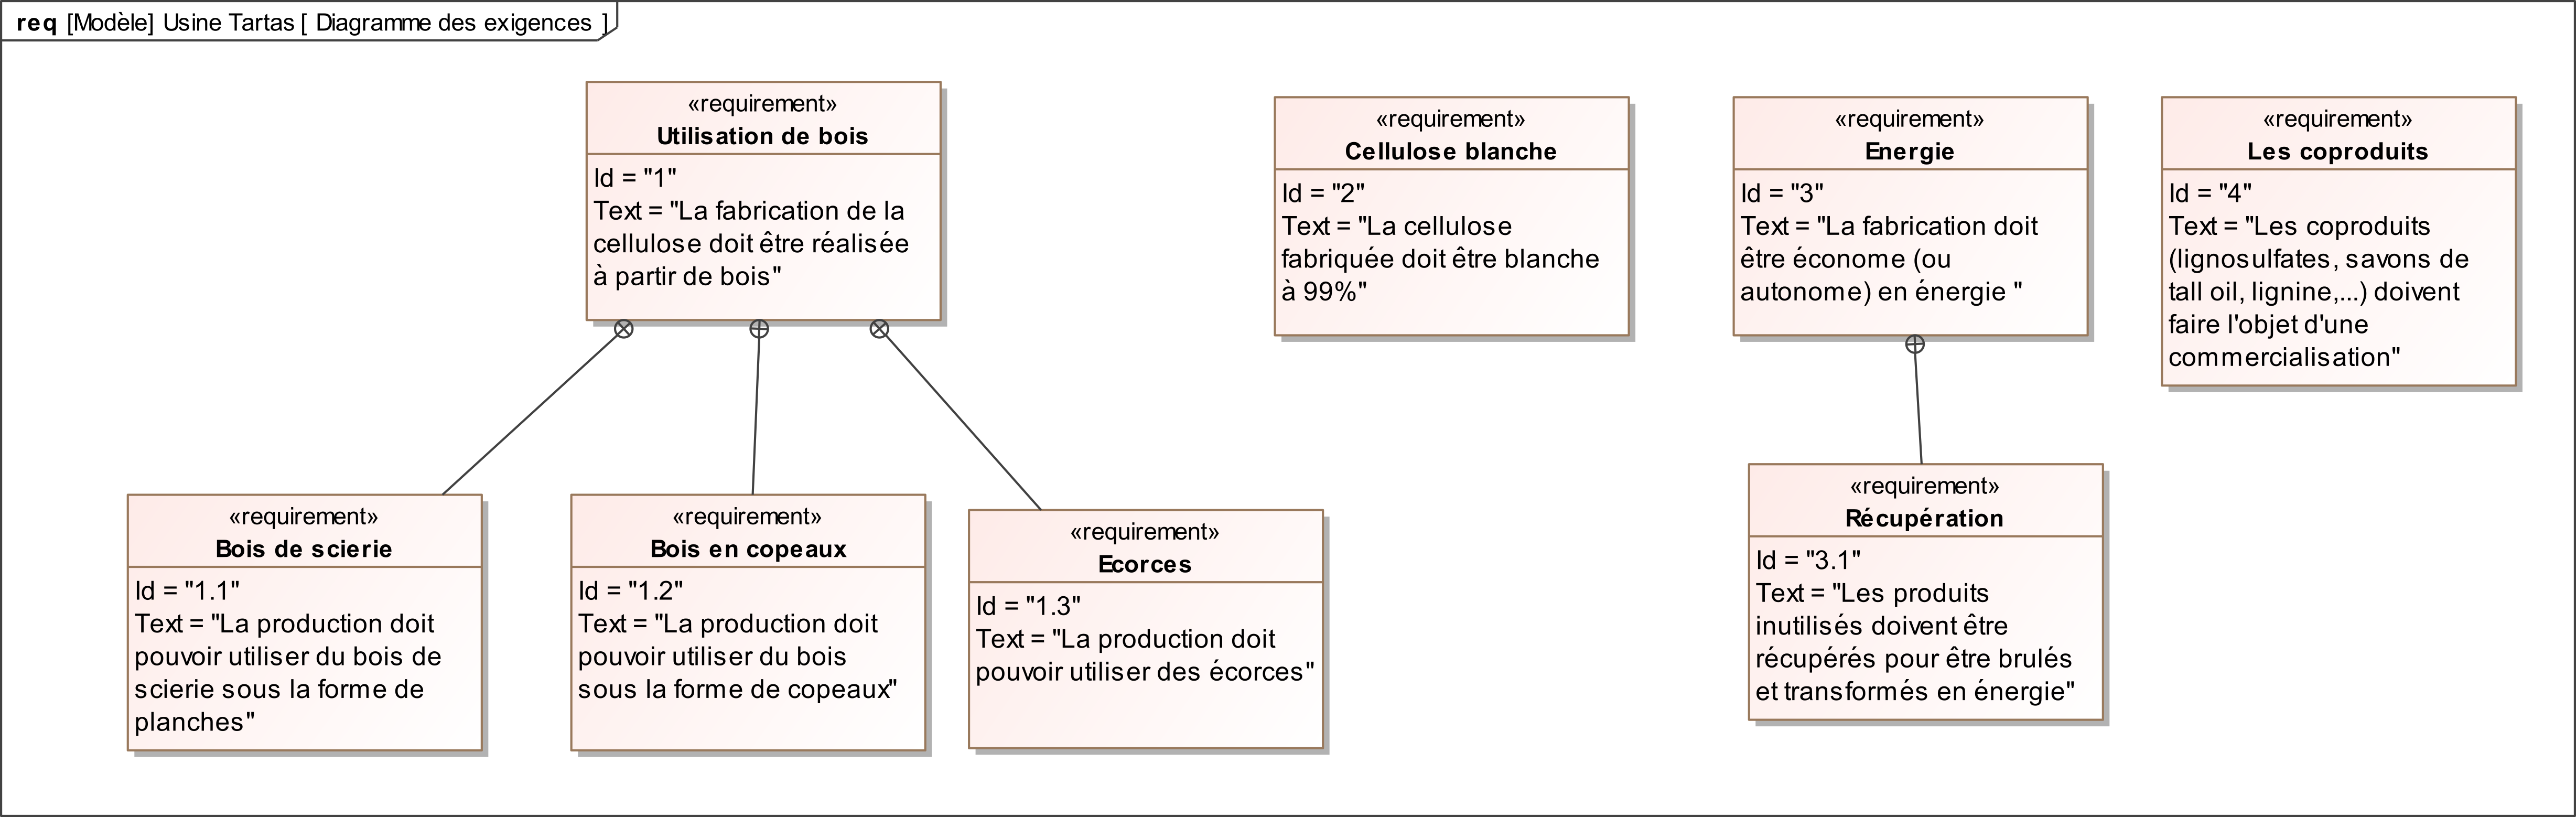
\includegraphics[width=\linewidth]{img/Tartas_exigences}
\caption{Diagramme des Exigences}
\label{fig:tartas_ex}
\end{center}
\end{figure}

\paragraph{Question 2:} Déterminer pour chaque exigence quels éléments du milieu extérieur sont à prendre en compte lors de son traitement.

~\

Le diagramme de définition de bloc de la figure \ref{fig:tartas_bl} présente un extrait de la liste des composants de l'entreprise.

\begin{figure}[!h]
\begin{center}
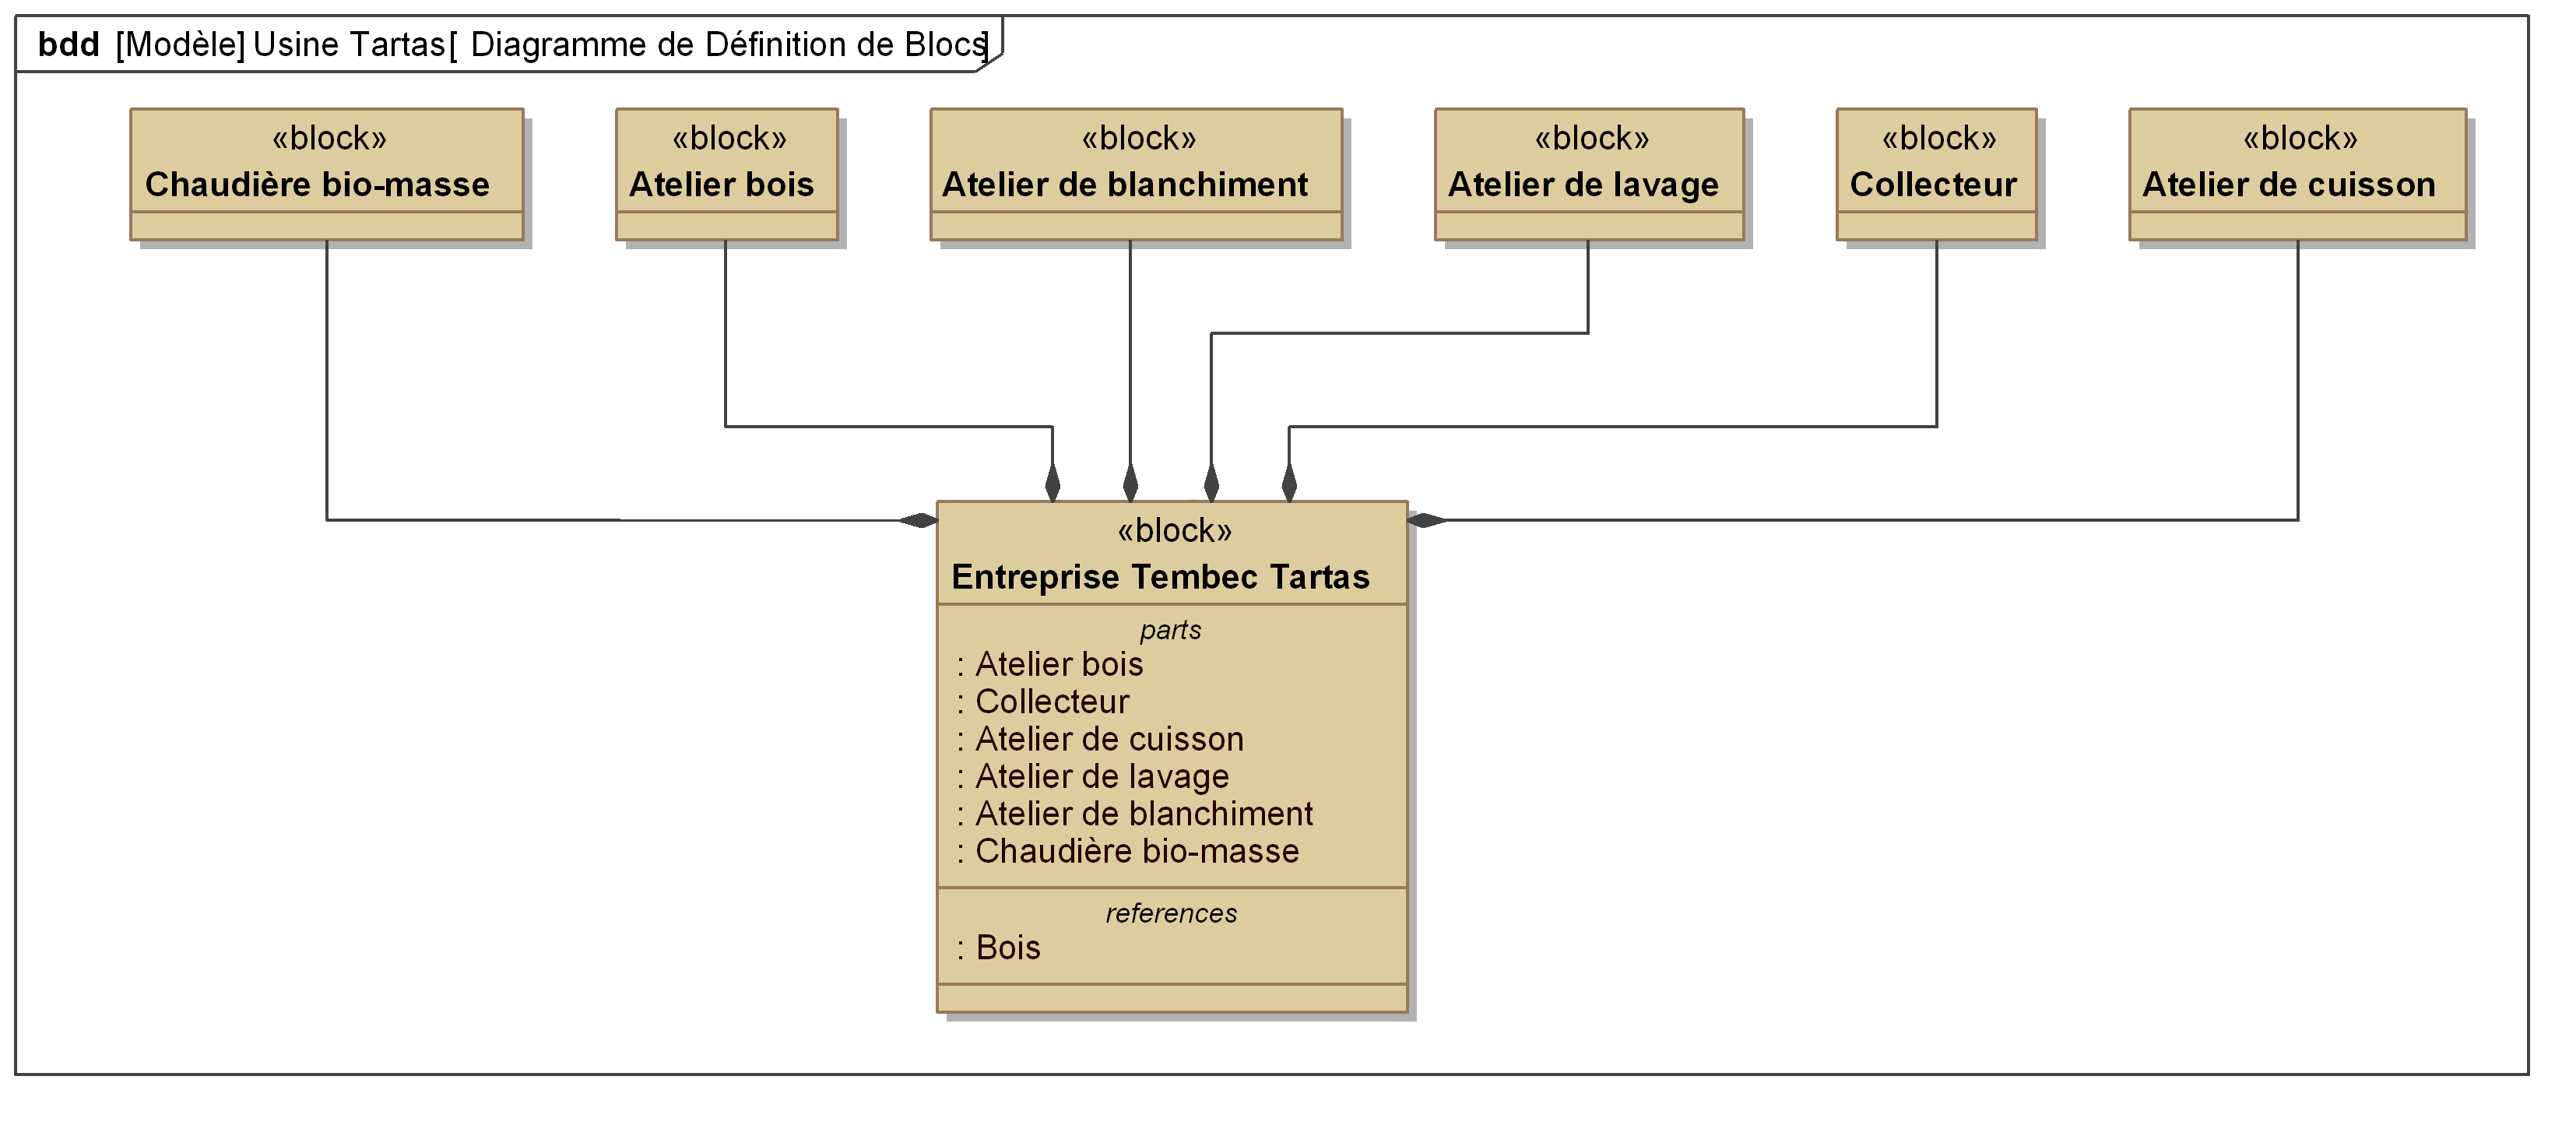
\includegraphics[width=\linewidth]{img/Tartas_bloc}
\caption{Diagramme de Définition de Bloc}
\label{fig:tartas_bl}
\end{center}
\end{figure}

Chaque composant présent sur le diagramme de la figure \ref{fig:tartas_bl} est une solution technique qui répond à une exigence.

\paragraph{Question 3:} Relier quand c'est possible la solution technique avec l'exigence à laquelle elle répond.

Lors de l'analyse des systèmes, ont a l'habitude de regrouper les composants selon qu'ils gèrent la fonction:
\begin{itemize}
 \item Alimenter: Produire ou récupérer de l'énergie afin de fournir le système en énergie compatible,
 \item Distribuer : Distribuer l'énergie au système en fonction des ordres de la partie commande (distributeur, contacteur,...),
 \item Convertir : Convertir l'énergie pour l'adapter à l'action à effectuer (vérin, moteur, résistance chauffante,...),
 \item Transmettre : Transmettre l'énergie aux système qui effectuent l'action (engrenages, courroies,...)
\end{itemize}

\paragraph{Question 4:} Compléter le tableau suivant en associant une fonction à chacun des sous-systèmes.

\begin{figure}[!h]
\begin{center}
\begin{tabular}{|c|c|c|c|c|c|}
\hline
& \textbf{Alimenter} & \textbf{Distribuer} & \textbf{Convertir} & \textbf{Transmettre} & \textbf{Agir}\\
\hline
Atelier bois & & x & x & x & x \\
\hline
Chaudière bio-masse & & & & & \\
\hline
Atelier de blanchiment & & & & & \\
\hline
Atelier de lavage & & & & & \\
\hline
Collecteur & & & & & \\
\hline
Atelier de cuisson & & & & & \\
\hline
\end{tabular}
\end{center}
\caption{Sous-systèmes/Chaîne d'énergie}
\end{figure}

Le Diagramme de bloc interne présenté à la figure \ref{fig:tartas_in} présente les flux qui traversent l'entreprise et qui relient chacun des composants.


\begin{figure}[!h]
\begin{center}
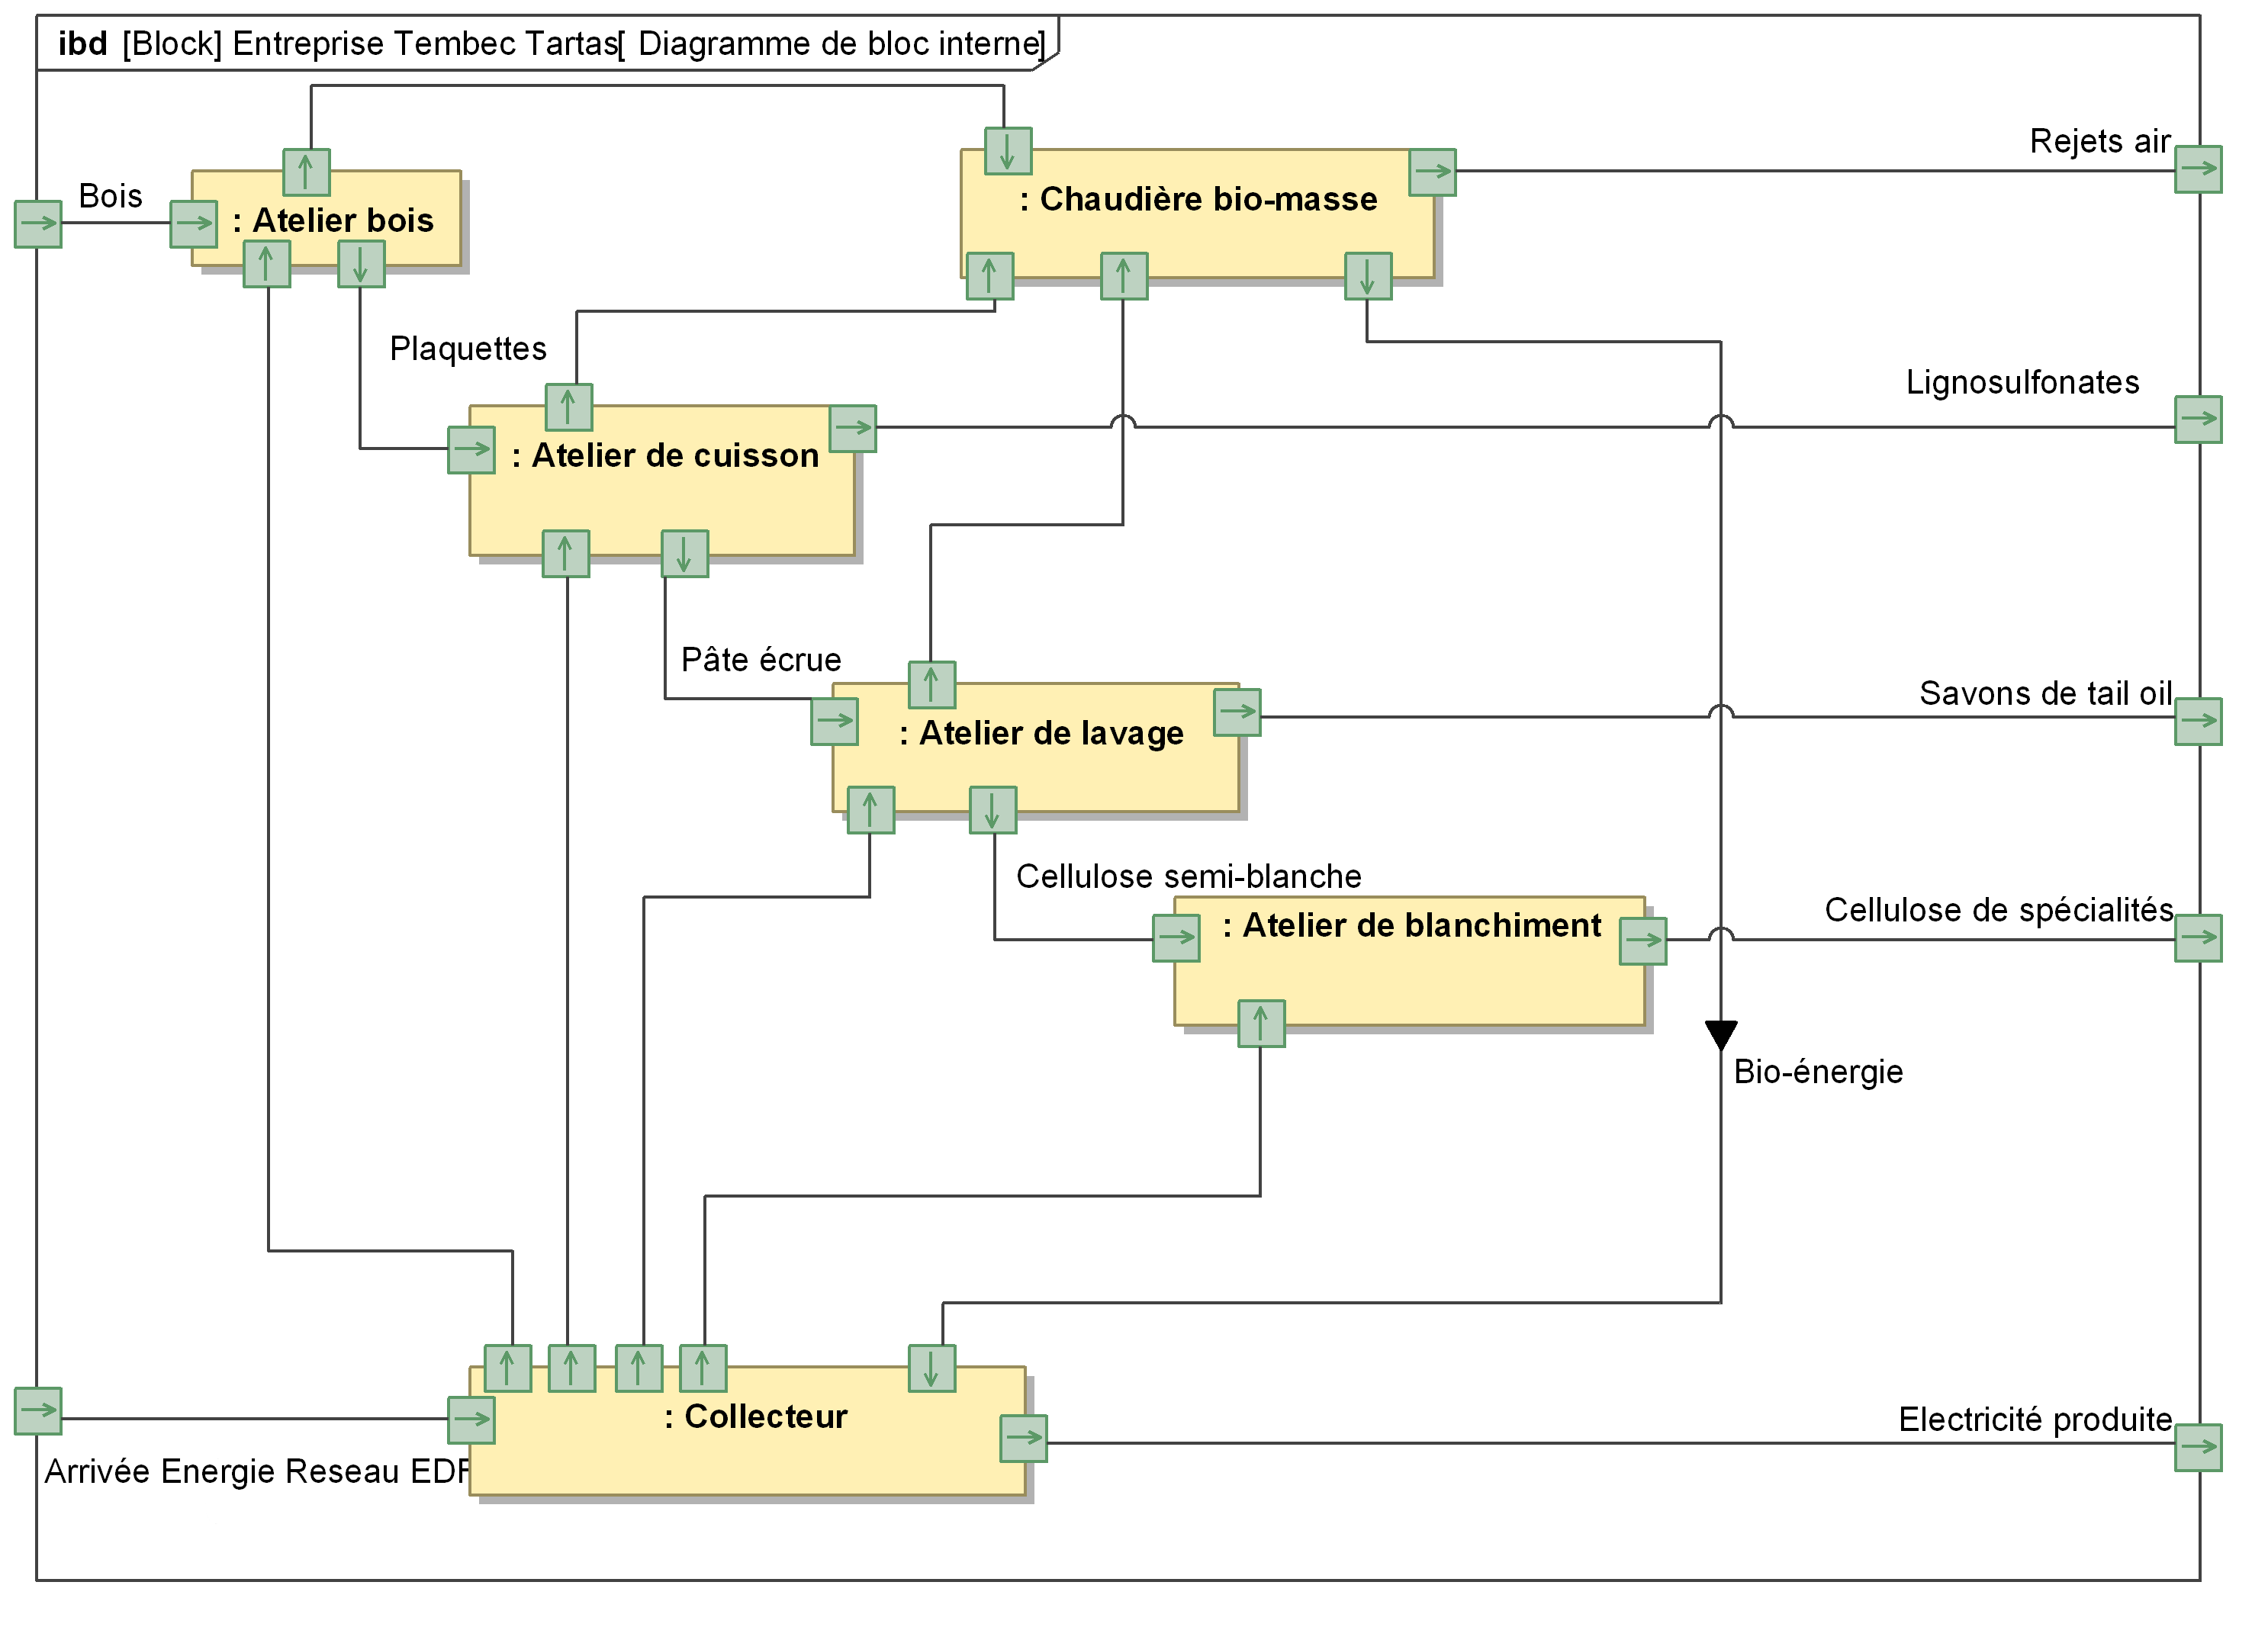
\includegraphics[width=\linewidth]{img/Tartas_interne}
\caption{Diagramme de Bloc Interne}
\label{fig:tartas_in}
\end{center}
\end{figure}

\paragraph{Question 5:} Colorier en vert les flux traversés par de la matière (bois, pâte, etc...), en rouge les flux traversés par de l'énergie et en bleu les flux traversés par les déchets à brûler.

\subsection{Étude d'éco-conception}

A la sortie de cette entreprise des co-produits sont fabriqués en plus des produits. 

\paragraph{Question 6:} Quels sont les produits ? Quels sont les co-produits ? Donner pour chacun le nom des acheteurs, et la quantité produite.

\newpage
\clearpage
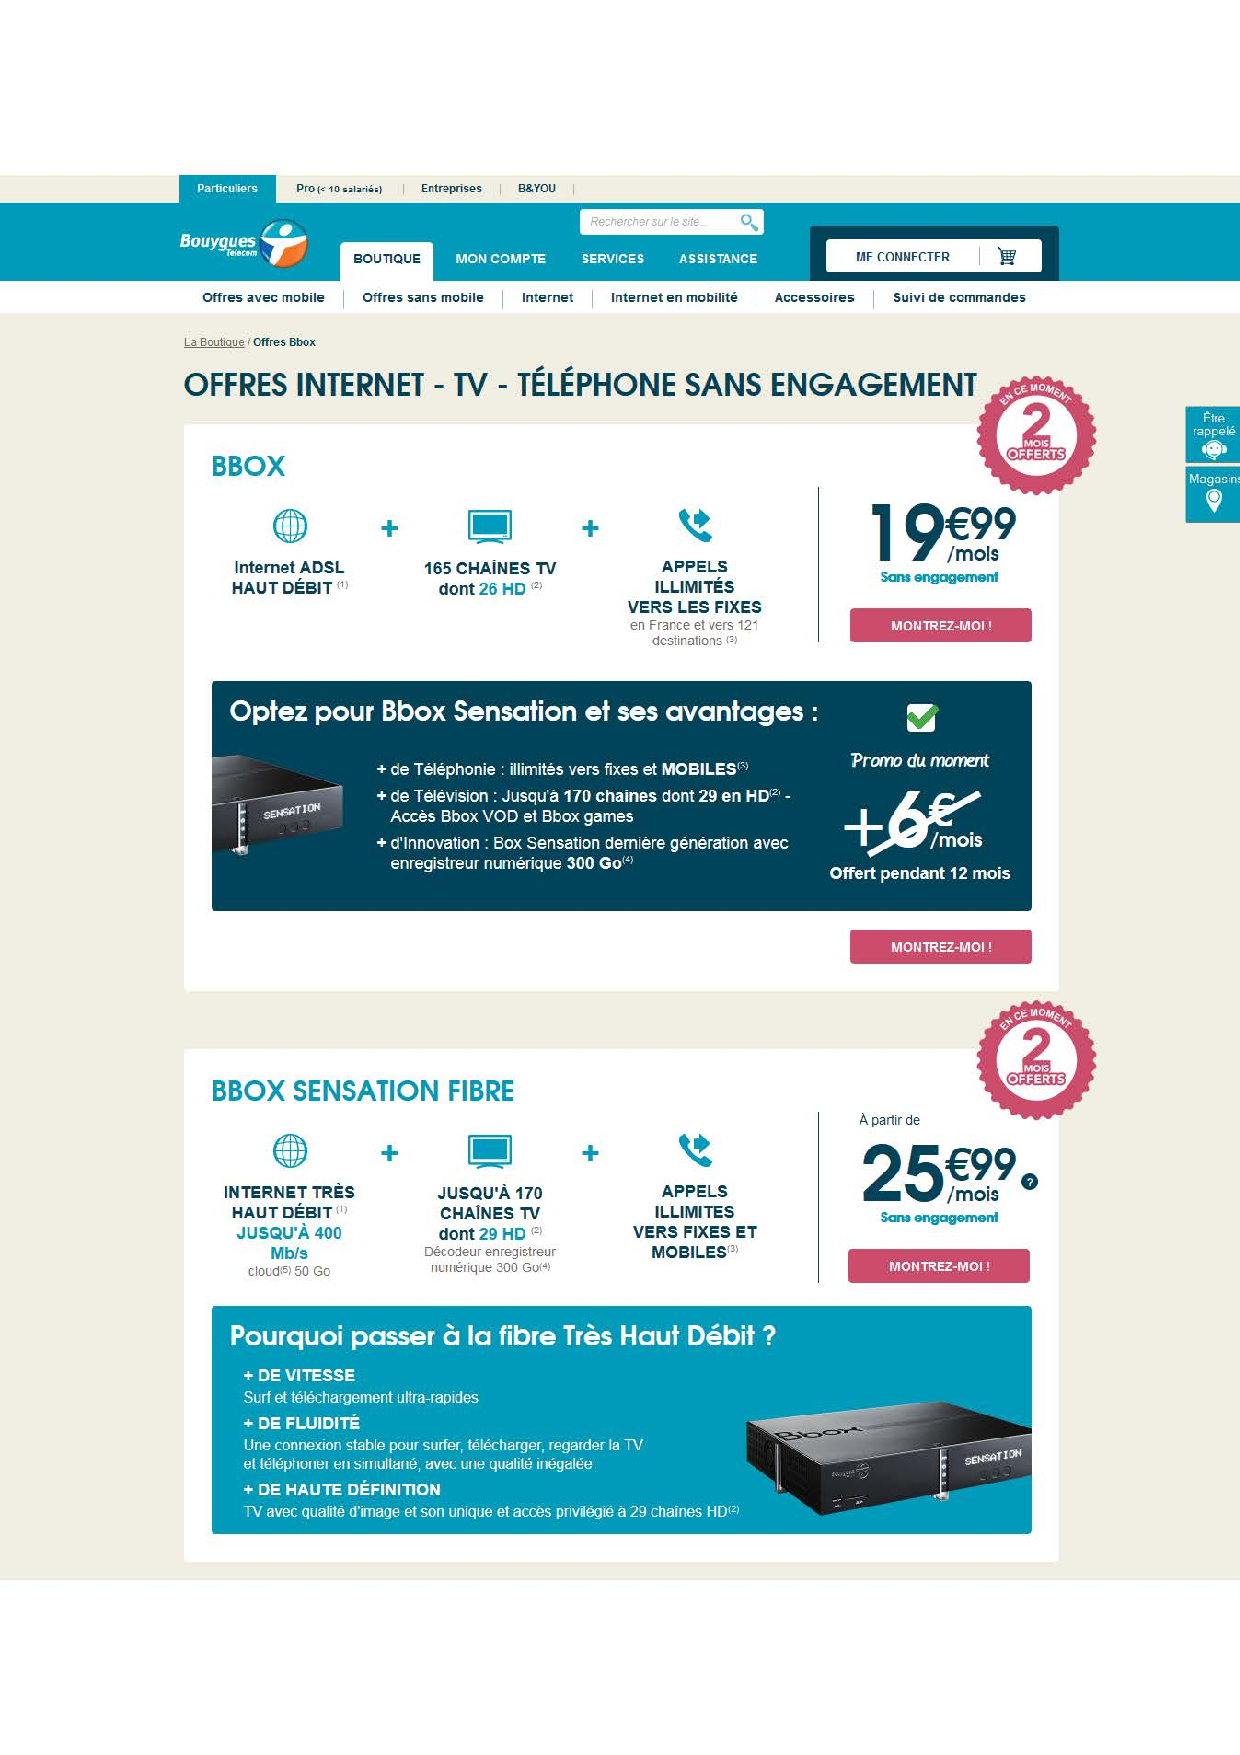
\includepdf[pages=1-9]{img/Sites_web.pdf}

\newpage

\begin{figure}
	\begin{center}
		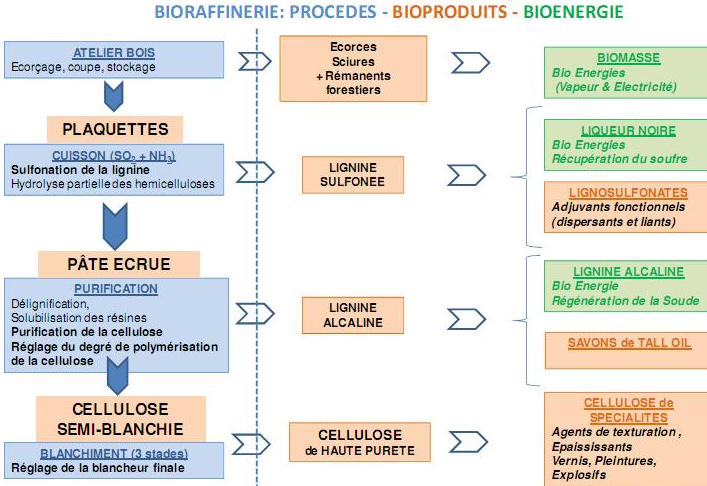
\includegraphics[width=0.8\linewidth]{img/processus.png}
		\caption{Processus de fabrication}
		\label{fig:processus}
		\vspace{2cm}
		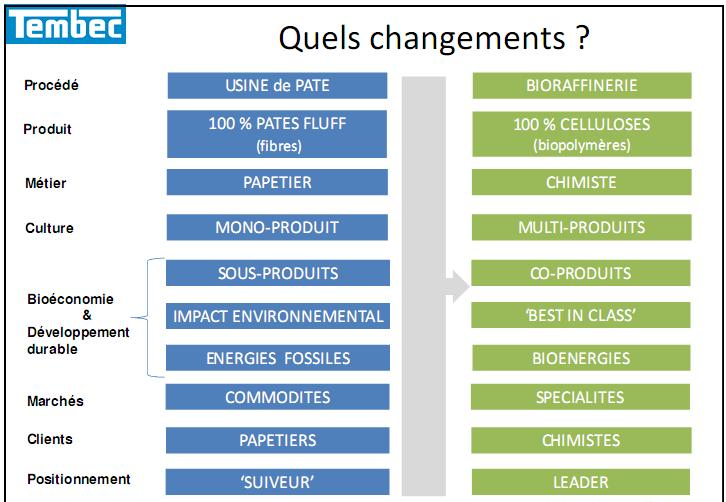
\includegraphics[width=0.8\linewidth]{img/changements.png}
		\caption{Changements dans la fabrication}
		\label{fig:changements}
	\end{center}
\end{figure}

\begin{figure}
	\begin{center}
		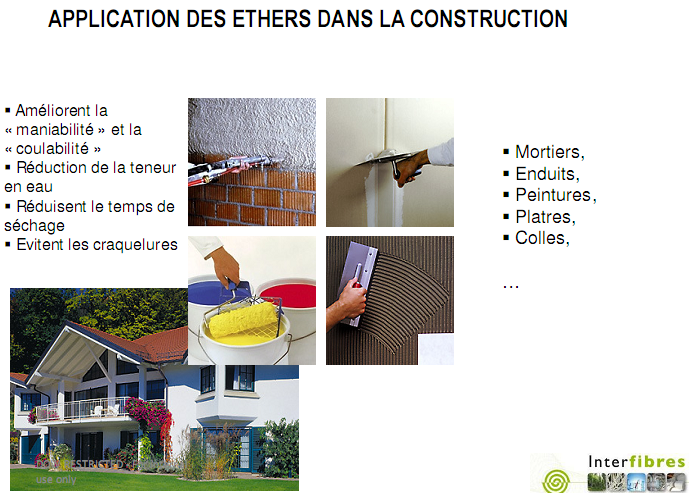
\includegraphics[width=0.8\linewidth]{img/applications.png} \\
		\vspace{2cm}
		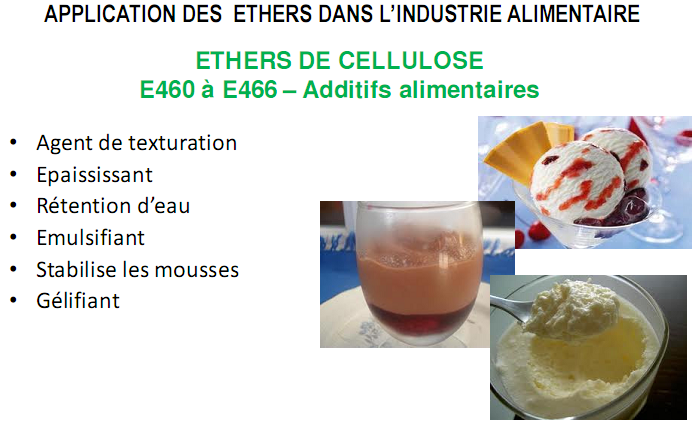
\includegraphics[width=0.8\linewidth]{img/applications2.png}
		\caption{Applications pour le produit}
		\label{fig:applications}
	\end{center}
\end{figure}

\begin{figure}
	\begin{center}
		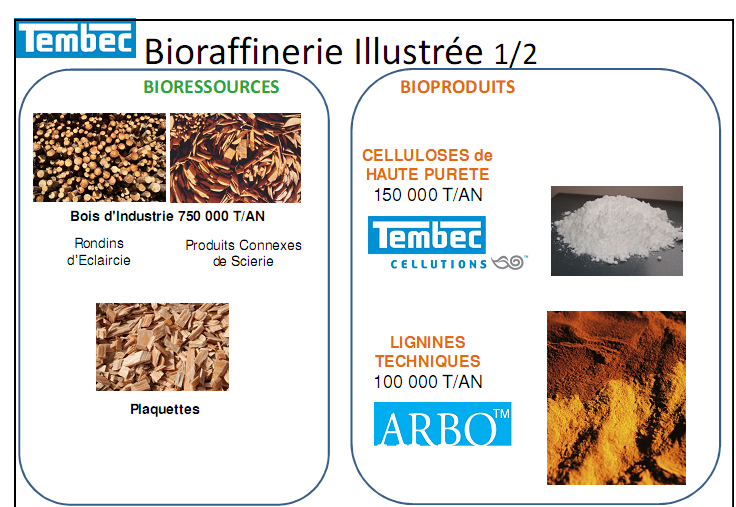
\includegraphics[width=0.8\linewidth]{img/bioproduits.png} \\
		\caption{Bio-produits}
		\label{fig:bioproduits}
	\end{center}
\end{figure}

\clearpage

\ifdef{\public}{\end{document}}{}

\newpage

\pagestyle{correction}

\section{Correction}

\subsection{Étude d'une Freebox}

\paragraph{Question 1:} Le nombre d'abonnés est de 5-6 millions.

\paragraph{Question 2:} Cette valeur est confirmée par la courbe, l'écart est de 6\%.

\paragraph{Question 3:} La courbe est croissante, le nombre d'abonnés a augmenté de 7\% en un an.

\paragraph{Question 4:} Free: le matériel (la box), les trois autres: les offres, services et prix.

\paragraph{Question 5:} L'acteur principal est l'utilisateur, l'ordinateur est acteur secondaire. Free (ou le réseau) peut être vu comme un acteur secondaire.

\paragraph{Question 6:} Ajout de cas d'utilisation : réponse libre.

\paragraph{Questions 7 et 8:} Pour le cas d'utilisation: \og Accéder à des chaînes numériques \fg, il faut les exigences 1, 1.2, 2 et 3 et les éléments externes sont: le réseau électrique, le réseau téléphonique, la télévision, utilisateur, la chaîne stéréo.

Pour le cas d'utilisation: \og Diffuser des contenus multimédias \fg, il faut les exigences 2, 3, 4, 4.1 et les éléments externes sont: le réseau électrique, le réseau téléphonique, la télévision, utilisateur, la chaîne stéréo, le PC.

Pour le cas d'utilisation: \og Passer des appels téléphoniques \fg, il faut les exigences 2 et 3 et les éléments externes sont: le réseau électrique, le réseau téléphonique, le téléphone.

Il faudra compléter le diagramme en fonction de la réponse 6.

\paragraph{Question 9:} 
\begin{itemize}
 \item Exigence 1: 2-3
 \item Exigence 1.1: 3 
 \item Exigence 1.2: 2
 \item Exigence 2: 1
 \item Exigence 3: 1
 \item Exigence 4: 4
 \item Exigence 4.1: 4 
\end{itemize}


\paragraph{Question 10:}

\begin{center}
 \begin{tabular}{|l|l|l|l|}
 \hline
 fabrication & transport & stockage & vente \\
 \hline
 utilisation & maintenance & recyclage & ... \\
 \hline
 \end{tabular}
\end{center}

\paragraph{Question 11:} Le réseau électrique, le réseau téléphonique. Les autres sont optionnels, cela dépend des services attendus par l’utilisateur.

\paragraph{Question 12:} Ce sont bien l'acteur et l’utilisateur.

\paragraph{Question 13:} Les acteurs impliqués sont l'utilisateur et l'ordinateur.

\paragraph{Question 14:} La télécommande a été utilisée à l'étape 3 et la freebox a marché jusqu'à présent. Le programme a été lancé sur l'ordinateur au départ et cela a été confirmé, donc le problème le plus probable serait un problème de communication entre le PC et la freebox.

L'ordinateur est un élément du milieu extérieur, il ne fait donc pas partie du système.

\subsection{Étude d'une entreprise: Tembec Tartas S.A.}

\paragraph{Question 1:} Les interacteurs sont le bois, le réseau EDF, l'environnement (eau, air, personnes,...), les clients, les employés, la direction,...

\paragraph{Question 2:} \textit{Plusieurs réponses sont possibles.}

Exigences 1, 1.1, 1.2, 1.3: Bois, employés, environnement, direction,....

Exigence 2: Client

Exigence 3: Réseau EDF, clients, direction, employés,...

Exigence 3.1: Clients, environnement,...

Exigence 4: Clients,...

\paragraph{Question 3:}

\begin{tabular}{|c|c|c|c|}
\hline
Ex 1 & Atelier bois & Ex 2 & Aterlier blanchiment/lavage \\
\hline
Ex 1.1 & Atelier bois & Ex 3 & Tous et surtout chaudière bio-masse \\
\hline
Ex 1.2 & Atelier bois & Ex 3.1 & Tous et surtout chaudière bio-masse \\
\hline
Ex 1.3 & Atelier bois & Ex 4 & Chaudière bio-masse, ateliers bois, cuisson et lavage \\
\hline
\end{tabular}

~\

\paragraph{Question 4:}

\begin{figure}[h!]
\begin{center}
\begin{tabular}{|c|c|c|c|c|c|}
\hline
& \textbf{Alimenter} & \textbf{Distribuer} & \textbf{Convertir} & \textbf{Transmettre} & \textbf{Agir}\\
\hline
Atelier bois & & x & x & x & x \\
\hline
Chaudière bio-masse & x & x & x & & \\
\hline
Atelier de blanchiment & & x & x & x & x \\
\hline
Atelier de lavage & & x & x & x & x \\
\hline
Collecteur & x & x & & & \\
\hline
Atelier de cuisson & & x & x & x & x \\
\hline
\end{tabular}
\end{center}
\caption{Sous-systèmes/Chaîne d'énergie}
\end{figure}

~\

\paragraph{Question 5:}


\begin{figure}[!h]
\begin{center}
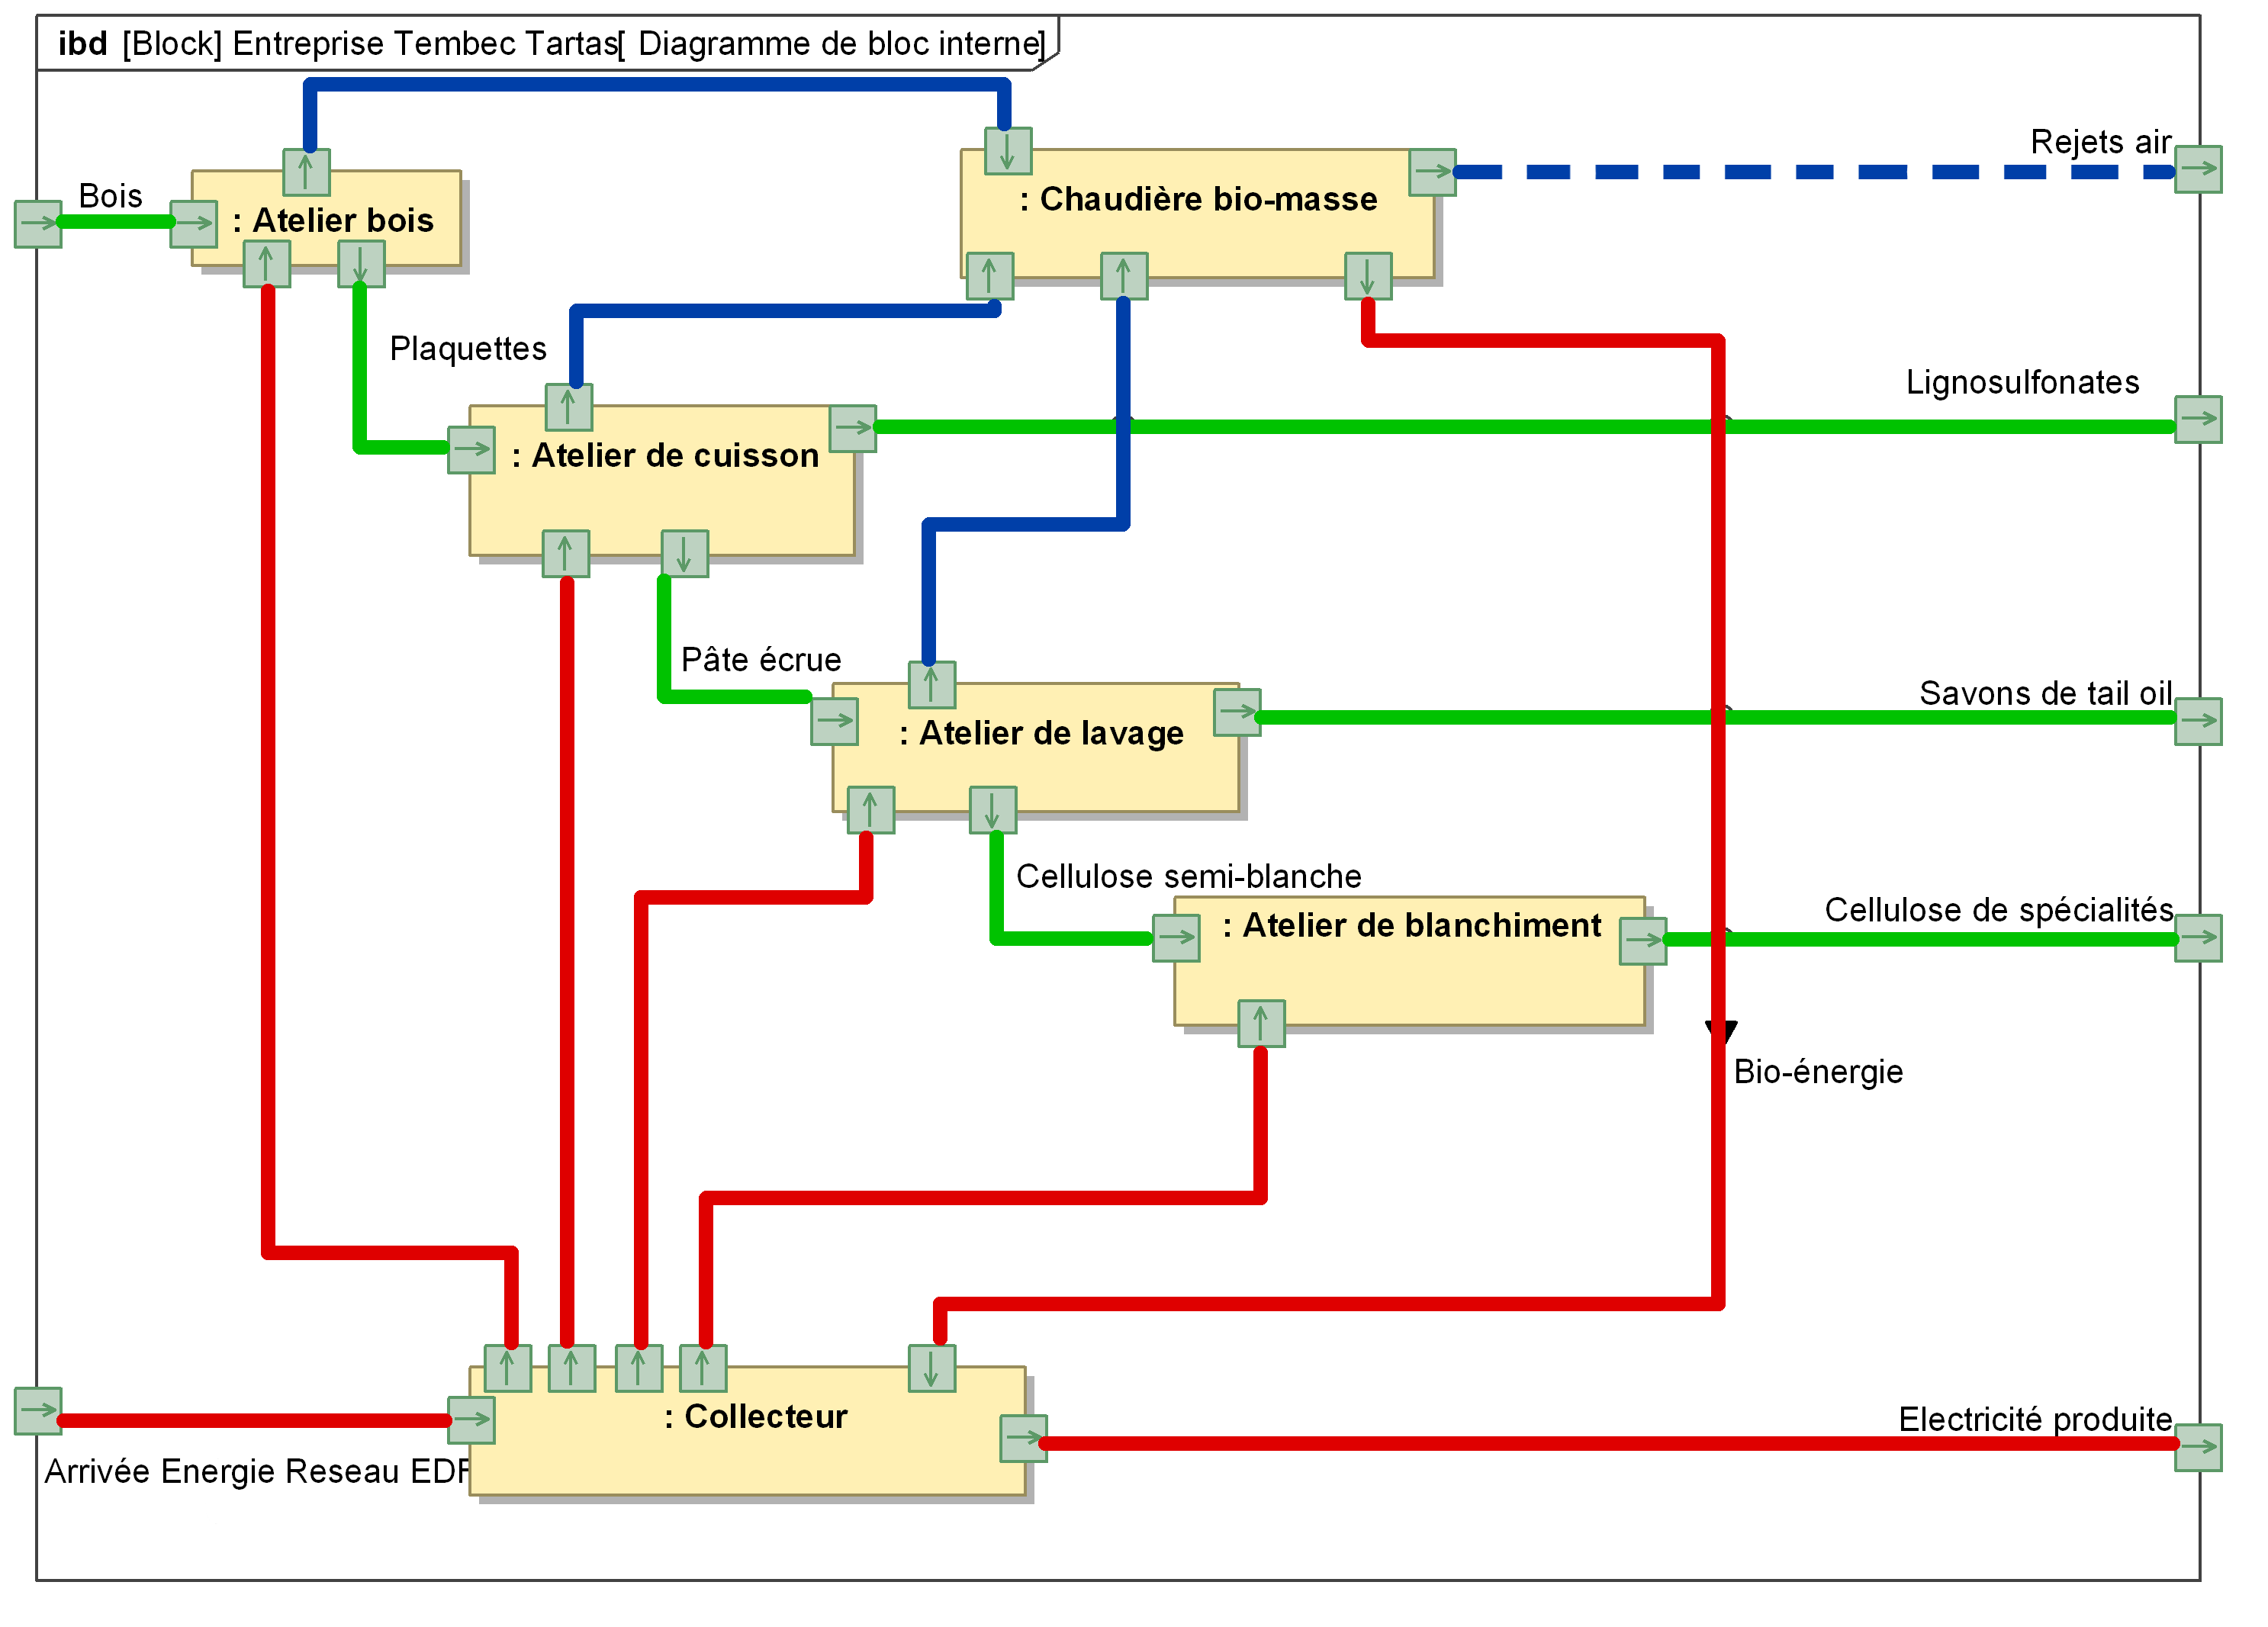
\includegraphics[width=\linewidth]{img/Tartas_interne_cor}
\caption{Diagramme de Bloc Interne corrigé}
\label{fig:tartas_in_cor}
\end{center}
\end{figure}


\paragraph{Question 6:} 

Produit : Celluloses de haute puretée

Co-produits: Lignosulfonates, savons de tail oil, électricité.

Cellulose: 150000Tonnes/an (Tembec Cellutions).

Lignines: 100000Tonnes/an (Arbo).

\end{document}
